%
%  ZanyBlue, an Ada library and framework for finite element analysis.
%
%  Copyright (c) 2012, Michael Rohan <mrohan@zanyblue.com>
%  All rights reserved.
%
%  Redistribution and use in source and binary forms, with or without
%  modification, are permitted provided that the following conditions
%  are met:
%
%    * Redistributions of source code must retain the above copyright
%      notice, this list of conditions and the following disclaimer.
%
%    * Redistributions in binary form must reproduce the above copyright
%      notice, this list of conditions and the following disclaimer in the
%      documentation and/or other materials provided with the distribution.
%
%    * Neither the name of ZanyBlue nor the names of its contributors may
%      be used to endorse or promote products derived from this software
%      without specific prior written permission.
%
%  THIS SOFTWARE IS PROVIDED BY THE COPYRIGHT HOLDERS AND CONTRIBUTORS
%  "AS IS" AND ANY EXPRESS OR IMPLIED WARRANTIES, INCLUDING, BUT NOT
%  LIMITED TO, THE IMPLIED WARRANTIES OF MERCHANTABILITY AND FITNESS FOR
%  A PARTICULAR PURPOSE ARE DISCLAIMED. IN NO EVENT SHALL THE COPYRIGHT
%  HOLDER OR CONTRIBUTORS BE LIABLE FOR ANY DIRECT, INDIRECT, INCIDENTAL,
%  SPECIAL, EXEMPLARY, OR CONSEQUENTIAL DAMAGES (INCLUDING, BUT NOT LIMITED
%  TO, PROCUREMENT OF SUBSTITUTE GOODS OR SERVICES; LOSS OF USE, DATA, OR
%  PROFITS; OR BUSINESS INTERRUPTION) HOWEVER CAUSED AND ON ANY THEORY OF
%  LIABILITY, WHETHER IN CONTRACT, STRICT LIABILITY, OR TORT (INCLUDING
%  NEGLIGENCE OR OTHERWISE) ARISING IN ANY WAY OUT OF THE USE OF THIS
%  SOFTWARE, EVEN IF ADVISED OF THE POSSIBILITY OF SUCH DAMAGE.
%

\chapter{The Text Package}
\label{chp:text}

The intent of the \texttt{Text} package is to allow the separate
definition of the text messages displayed by an application into a
\texttt{.properties} file.  Messages are reference in the source code
by a key value (a simple string or accessor function returning the text
associated with a particular key) within a group of related messages---a
facility.  The message strings include Java style message argument
place holders: argument number (zero-based) along with optional type specific
formatting information enclosed in chain brackets.  Allowing formatting
of message arguments in the context of a localized message.

The divorce of the message text from the source code allows the easy
localization of application messages.  The source language \texttt{.properties}
file is delivered to translation vendors who then return localized
\texttt{.properties} files.  E.g., for an application \texttt{myapp}, with
application messages defined in the file
\begin{verbatim}
    myapp.properties
\end{verbatim}
the localized French and Japanese files would be
\begin{verbatim}
    myapp_fr.properties
    myapp_ja.properties
\end{verbatim}

The \texttt{Text} package supports message text searching among a set of
localized \texttt{.properties} files with fallback to available messages.
For example, if the above application, \texttt{myapp}, is run in a Canadian
French environment (\texttt{ZB\_LANG=fr\_CA}), localized display of each message
is implemented by trying to locate the message in the files, in order,
\begin{verbatim}
    myapp_fr_CA.properties
    myapp_fr.properties
    myapp.properties
\end{verbatim}
If no French localized message is available, the source development language
message text is used, i.e., the properties file which does not include a
language code.  Frequently this is English.

\section{Messages and Arguments}

The localization of a message cannot, in general, occur using just the
text `snippets' surrounding values generated by an application, e.g., the
externally visible message
\begin{verbatim}
    There are 2 moons orbiting "Mars".
\end{verbatim}
could be divided into the `snippets'
\begin{itemize}
\item ``\texttt{There are}''
\item ``\texttt{moons orbiting}''
\item ``\texttt{.}''
\end{itemize}
concatenated together at runtime along with formatted values for the number
of moons and the planet name.
If delivered to a translation vendor, the `snippet' would needs to localize
independently. This is a rather
difficult task to do for general text `snippets' as the order of the
`snippets' is defined by the application and cannot be changed by localization
vendors.  The `snippets' themselves are generally too short to give
translators sufficient context.  As a general rule, translation should be
performed on complete sentences.

A complete sentence is possible if place holders are used for message
arguments.  Using Java style arguments, the above message would be defined as
\begin{verbatim}
    There are {0} moons orbiting "{1}".
\end{verbatim}
The application message arguments are referenced within chain brackets.
In the example here, argument 0 would be the integer \texttt{2} and argument
1 would be the string``\texttt{Mars}''.

This message is then stored in a \texttt{.properties} file, external to the
application and given a key name, e.g., to use they key string
``\texttt{moons}'' to refer to the message in the application code, the
\texttt{.properties} file definition
would be
\begin{verbatim}
    moons=There are {0} moons orbiting "{1}".
\end{verbatim}

This sentence can be localized independently of the application and, since
the English string is also defined externally to the application, this
text can also be changed.  For example, if a technical writer review of the
English used in an application decided, for consistency reasons, to rephrase
the sentence, just the English properties file need be adjusted, e.g.,
\begin{verbatim}
    moons=The planet "{1}" has {0} moons.
\end{verbatim}

This model of searching \texttt{.properties} files is a conceptual model in the
context of the ZanyBlue Text library.  The ZanyBlue implementation compiles
the set of properties files for a facility into Ada code and localized message
resolution for a particular key occurs against run-time data structures rather
than accessing files.  This makes for an efficient implementation where the
major portion of the data processing occurs at application build time.  See
details on the \texttt{zbmcompile} (\ref{sec:zbmcompile}), the ZanyBlue message
compiler, later.

\section{Example Using Low Level Functions}

As an introduction to the \texttt{Text} package, a simple example, which
continues the example based on the number of moons orbiting the various
planets, is developed here.

\textbf{Note}, the preferred way to access messages is using accessor
packages described in the next section.   The example here uses direct
calls using strings to identify facilities and key to demonstrate the
concepts involved.

The task is to ask the user for a planet name and print the number of currently
known moons for the planet.  The source for this simple example
is available in the directory \texttt{examples/text/moons} and is listed here:
\begin{xmpl}
\begin{verbatim}
with Ada.Wide_Text_IO;
with Moons_Messages;
with ZanyBlue.Text.Formatting;

procedure Moons is

   type Planet_Names is (Mercury, Venus, Earth, Mars,
                         Jupiter, Saturn, Uranus, Neptune);
   package Planet_Name_IO is
      new Ada.Wide_Text_IO.Enumeration_IO (Planet_Names);

   use Ada.Wide_Text_IO;
   use Planet_Name_Formatting;
   use ZanyBlue.Text.Formatting;

   Moons  : array (Planet_Names) of Natural := (
                   Earth => 1, Mars => 2, Jupiter => 63,
                   Saturn => 62, Uranus => 27, Neptune => 13,
                   others => 0);
   Planet : Planet_Names;

begin
   loop
      Print ("moons", "0001");
      Planet_Name_IO.Get (Planet);
      if Moons (Planet) /= 1 then
         Print_Line ("moons", "0002", +Moons (Planet),
                                      +Planet_Names'Image (Planet));
      else
         Print_Line ("moons", "0003", +Planet_Names'Image (Planet));
      end if;
   end loop;
exception
when End_Error | Data_Error =>
    New_Line;
    Print_Line ("moons", "0004");
end Moons;
\end{verbatim}
\end{xmpl}
The example source code uses the \texttt{Generic\_Enumerations} ZanyBlue
package for planet name arguments.  Generic ZanyBlue packages should
be instanciated at the library level.

Here the messages for the application are referred to by message id or
key, i.e., numeric strings, e.g., ``\texttt{0001}'' for the facility
``\texttt{moons}''.\footnote{As a side note, the key is a general string,
however, the assignment of more meaningful names becomes more difficult
as an application grows and it is simpler to abandon such names initially
and use numeric string codes.}
The text associated with these message keys are externalized to a
\texttt{.properties} file.  For this example, the root properties file,
``\texttt{moons.properties},'' containing English, is
\begin{xmpl}
\begin{verbatim}
   0001=Please enter a planet:
   0002=There are {0} known moons orbiting "{1}".
   0003=There is 1 known moon orbiting "{0}".
   0004=OK, goodbye.
\end{verbatim}
\end{xmpl}

A German translation of this properties, ``\texttt{moons\_de.properties}'',
file would be (via Google Translate)
\begin{small}
\begin{verbatim}
   0001=Bitte geben Sie einen Planeten:
   0002=Es gibt {0} bekannte Monde umkreisen "{1}".
   0003=Es gibt 1 bekannt Mond umkreisen "{0}".
   0004=OK, auf Wiedersehen.
\end{verbatim}
\end{small}
French and Spanish Google translated version of this file in the examples
directory.

The properties and application are tied together by ``compiling'' the
properties files into an Ada package and simply \textbf{with}'ing the
compiled package in the application (normally in the unit containing
the main procedure).  In this example, the generated package referenced
in the source above is \texttt{Moons\_Messages} which is created using
the \texttt{zbmcompile} ZanyBlue message compiler utility:
\begin{xmpl}
\begin{verbatim}
   $ zbmcompile -i -v Moons_Messages moons
   This is ZBMCompile, Version 1.0.0 BETA (r2621) at 8:25:33 AM on Feb 23, 2012
   Copyright (c) 2009-2012, Michael Rohan.  All rights reserved
   Loaded 16 messages for the facility "moons" (4 locales)
   Performing consistency checks for the facility "moons"
   Loaded 1 facilities, 4 keys, 4 locales and 16 messages
   Loaded total 517 characters, stored 517 unique characters, 0% saving
   Wrote the spec "Moons_Messages" to the file "./moons_messages.ads"
   Wrote the body "Moons_Messages" to the file "./moons_messages.adb"
   ZBMCompile completed at 8:25:33 AM on Feb 23, 2012, elapsed time 0:00:00.057
\end{verbatim}
\end{xmpl}

This generates an Ada specification containing the name of the facility,
``moons'' in this case, and the definition of a single initialization routine.
The body file contains the message text data, the initialization routine which
adds the message data to a shared message pool.  Since the \texttt{-i}
command line option was used, the generated package body includes a call
to the initialization routine allowing the message data to be included
in the application via a simple \textbf{with} of the package, i.e., no
explicit call to the initialization routine is needed.

The execution of the generated application will now display messages selected
for the run-time locale, e.g., in an English locale:
\begin{xmpl}
\begin{verbatim}
    $ make run
    ../../../bin/x_moons
    Please enter a planet: mars
    There are 2 known moons orbiting "MARS".
    Please enter a planet: earth
    There is 1 known moon orbiting "EARTH".
    Please enter a planet: mercury
    There are 0 known moons orbiting "MERCURY".
    Please enter a planet: ^D
    OK, goodbye.
\end{verbatim}
\end{xmpl}

And running the application selecting a German locale displays the German
messages:
\begin{xmpl}
\begin{verbatim}
    $ make run_de
    ../../../bin/x_moons de
    Bitte geben Sie einen Planeten: mars
    Es gibt 2 bekannte Monde umkreisen "MARS".
    Bitte geben Sie einen Planeten: earth
    Es gibt 1 bekannt Mond umkreisen "EARTH".
    Bitte geben Sie einen Planeten: mercury
    Es gibt 0 bekannte Monde umkreisen "MERCURY".
    Bitte geben Sie einen Planeten: ^D
    OK, auf Wiedersehen.
\end{verbatim}
\end{xmpl}
The locale is selected via a command line argument here, however, the
environment variables can be used instead, see section~\ref{sec:changelocale}
for more details on selecting locales.

This example application did not attempt to localize the planet names.  A
more involved example would add another facility for the planet names with
message keys matching the \texttt{Image} of the enumeration values.

\section{Example Using Accessor Functions}

The style of message generation using a facility string, key string and
message arguments opens an application up to the risk of a mis-match between
the expected arguments for a message and the supplied arguments (possibly
causing the ZanyBlue exceptions \texttt{No\_Such\_Argument\_Error} or
\texttt{No\_Such\_Key} to be raised).  It is also possible to silently, in
the sense the compiler does not compile, introduce errors by accidentally
mis-spelling a facility or key value (again possibly causing the exceptions
\texttt{No\_Such\_Facility\_Error} \texttt{No\_Such\_Key\_Error} to raised).

For an Ada application, where the compile time detection of errors is an
expection, this is not ideal.  To overcome this, the ZanyBlue message
compiler utility can generate accessor packages for the compiled facilities.
These packages define functions and procedures for each key in the facility
with a list of arguments matching the expected number of arguments.  This
allows the Ada compiler to perform checks on the references to messages of
ZanyBlue-ised applications.

The \texttt{zbmcompile} utility generates three major classes of accessor
packages (when the \texttt{-a} option is given):
\begin{enumerate}
\item	Accessor functions which return the localized formatted message for
	a message key.  There are two accessor function packages generated:
	\begin{itemize}
	\item	A package for functions with return typed of
	 	\texttt{Wide\_String}.
	\item	A package for functions with return typed of \texttt{String}
		(the standard Wide Strings are UTF-8 encoded in this case).
	\end{itemize}
	In both cases, the functions generated are named by using message key
	prefixed with the string ``\texttt{Format\_}''.  This requires message
	keys be valid Ada identifier characters.
\item   Accessor that print the localized formatted message similar to the
        standard \texttt{Put\_Line} routines.  There are two styles of routines
        generated:
        \begin{itemize}
        \item Routines that use the standard \texttt{Ada.Wide\_Text\_IO}
              routines to print the formatted messages.
        \item Routines that use the standard \texttt{Ada.Text\_IO}
              routines to print the formatted messages as UTF-8 encoded
              strings.
        \end{itemize}
\item	Accessor procedures which raise an exception with a localized formatted
	message (similar to the standard \texttt{Raise\_Exception} procedure
	but extended to allow message arguments).  The procedures names
	generated prefix the message key with the string ``\texttt{Raise\_}''.
\end{enumerate}

These accessor packages are generated for each facility compiled and are
created as child packages of the command line package name.

As an example, reworking the moons example in terms of the safer accessor
functions, the code would be, e.g., for the message that prints the number
of moons for a planet, using the generated wide print routine:
\begin{xmpl}
\begin{verbatim}
    with Messages.Moons_Wide_Prints;
    ...
    Print_0002 (+Moons (Planet), +Planet));
\end{verbatim}
\end{xmpl}
Here, the compiled messages are generated to the \texttt{Messages} package
and the accessor packages are child packages of it.

For this accessor example, the \texttt{zbmcompile} utility must be used with
the ``\texttt{-a}'' command line option to generate the accessor packages and
the target parent package is given as ``\texttt{Messages}'':
\begin{xmpl}
\begin{verbatim}
  $ zbmcompile -a -i -v Messages Moons
  This is ZBMCompile, Version 0.2.0 ALPHA (r2621) at 8:58:04 AM on Feb 21, 2012
  Copyright (c) 2009-2012, Michael Rohan.  All rights reserved
  Loaded 18 messages for the facility "Moons" (4 locales)
  Performing consistency checks for the facility "Moons"
  Performing consistency checks for the accessor package generation
  Loaded 1 facilities, 5 keys, 4 locales and 18 messages
  Loaded total 551 characters, stored 551 unique characters, 0% saving
  Wrote the spec "Messages" to the file "./messages.ads"
  Wrote the body "Messages" to the file "./messages.adb"
  Generated accessor package spec "Messages.Moons_Exceptions"
      to "./messages-moons_exceptions.ads"
  Generated accessor package body "Messages.Moons_Exceptions"
      to "./messages-moons_exceptions.adb"
  Generated accessor package spec "Messages.Moons_Strings"
      to "./messages-moons_strings.ads"
  Generated accessor package body "Messages.Moons_Strings"
      to "./messages-moons_strings.adb"
  Generated accessor package spec "Messages.Moons_Wide_Strings"
      to "./messages-moons_wide_strings.ads"
  Generated accessor package body "Messages.Moons_Wide_Strings"
      to "./messages-moons_wide_strings.adb"
  Generated accessor package spec "Messages.Moons_Prints"
      to "./messages-moons_prints.ads"
  Generated accessor package body "Messages.Moons_Prints"
      to "./messages-moons_prints.adb"
  Generated accessor package spec "Messages.Moons_Wide_Prints"
      to "./messages-moons_wide_prints.ads"
  Generated accessor package body "Messages.Moons_Wide_Prints"
      to "./messages-moons_wide_prints.adb"
  ZBMCompile completed at 8:58:04 AM on Feb 21, 2012, elapsed time 0:00:00.176
\end{verbatim}
\end{xmpl}
(Long output lines have been wrapped).

The minor difference in the naming of the properties files should also be
noted: for the example in the previous section, the files, and hence the
facility, were all lower case.  Here, the base file name is ``Moons''.
This allow the generated Ada packages to have the more expected name
``\texttt{Moons\_Wide\_Strings}''.

Since the messages are now, in a sense, handled by the Ada compiler, IDE's,
e.g., GPS, will display the message text (the generated packages include the
message text, with markers explained later).  The accessor display in GPS
for the example message above is given in figure~\ref{fig:moons-accessor}.
\begin{figure}
\begin{center}
\begin{latexonly}
    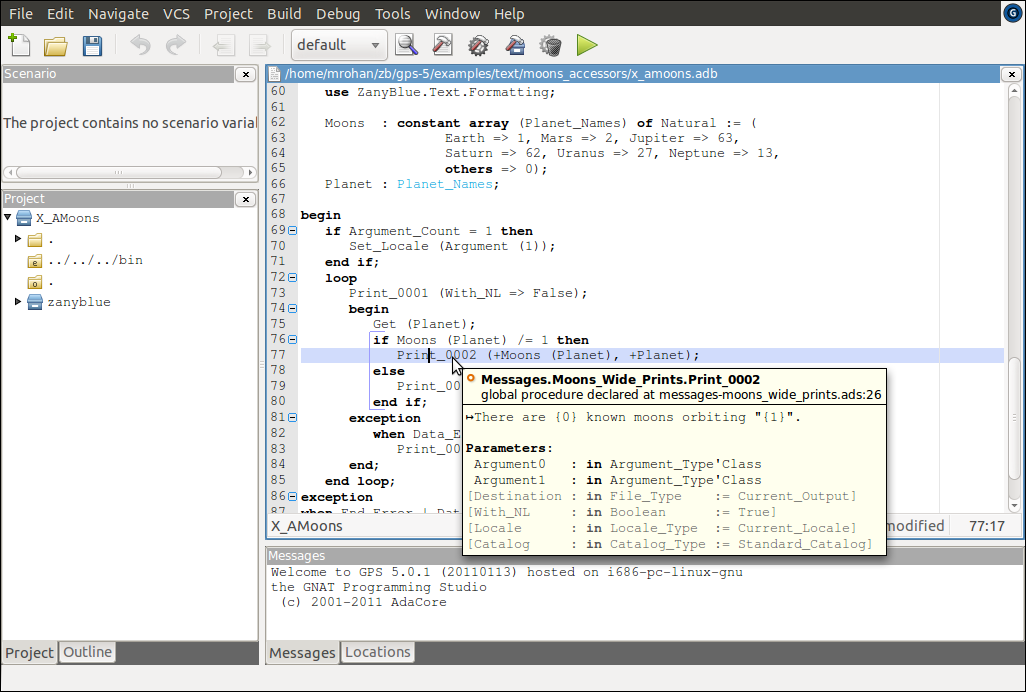
\includegraphics[angle=90,width=4in]{images/gps-accessor.png}
\end{latexonly}
\begin{htmlonly}
    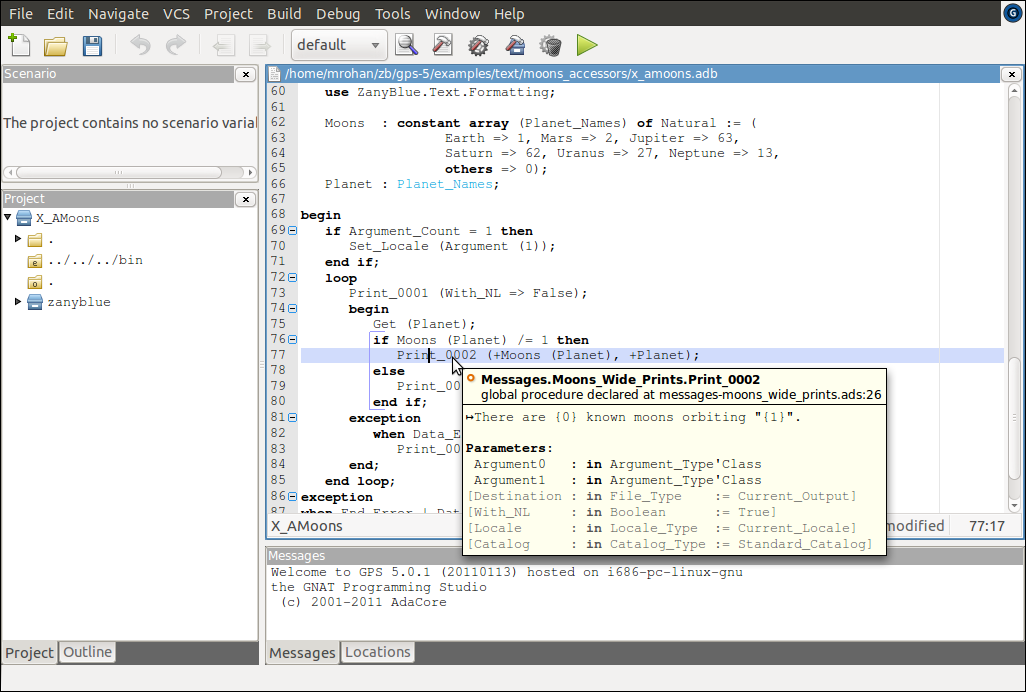
\includegraphics[width=4in]{images/gps-accessor.png}
\end{htmlonly}
\end{center}
\caption{GPS display for an accessor function.}
\label{fig:moons-accessor}
\end{figure}
The keys used for the messages in this example are simple numeric style
strings.  The GPS IDE will also display the base language text and
the number of arguments expected for accessors as the generated Ada code
includes this text as a comment.

\section{Message Formatting}

From the simple ``moons'' example above, it can be seen that simply
externalizing just the text used to in an application without the argument
formatting is not enough to fully support localization.  The messages
externalized must be the complete messages, i.e., sentences, with embedded
place holders for the arguments substituted at runtime.

The ZanyBlue Text library currently uses a mixture of Java and Python styles
for embedded arguments.  Arguments to the message are referenced by index
(zero based) and enclosed in chain brackets.

From the ``moons'' example, message ``\texttt{0002}'' has the definition
\begin{xmpl}
\begin{verbatim}
   0002=There are {0} known moons orbiting "{1}".
\end{verbatim}
\end{xmpl}

Here the first argument (argument 0) is an integer and second argument
(argument 1) is an enumeration value giving the planet name.

At runtime, arguments to messages are ``boxed'' into a tagged type with
dispatching methods that perform the formatting to strings.  Each type has
it's own implementation (see ``Provided Argument Types'' later,
\ref{sec:argtypes}).  Boxing occurs by creating a boxed object for the
argument value and passed to the various message formatting or printing
routines.  The boxing function has a standard ``\texttt{Create}'' function
and a renaming ``\texttt{+}'' making formatting or printing calls look more
natural.  For example, the message text above could be formatted with an
integer argument, 2, and a string argument, ``Mars'', as
\begin{xmpl}
\begin{verbatim}
    Message : Wide_String := Format ("moons", "0002", +2, +String'("Mars"));
\end{verbatim}
\end{xmpl}
or, if the accessor package is used,
\begin{xmpl}
\begin{verbatim}
    Message : Wide_String := Format_0002 (+2, +String'("Mars"));
\end{verbatim}
\end{xmpl}
The explicit type coercion to \texttt{String} is required as both standard
\texttt{String} and \texttt{Wide\_String} are supported.

The formatting or printing routines accept up to 5 optional boxed arguments.
The implementation gathers the supplied boxed arguments into an argument
list and then calls the underlying formatting routine with the argument
list.  For argument numbers beyond 5, the underlying argument list type must be
used and the arguments must be explicitly appended, e.g., the above
example could be rephrased in terms of the lower level argument list based
formatting routine as
\begin{xmpl}
\begin{verbatim}
   declare
      Arguments : Argument_List;
   begin
      Arguments.Append (1);
      Arguments.Append (String'("Mars"));
      Display_Message (Format ("moons", "0002", Arguments));
   end;
\end{verbatim}
\end{xmpl}

This 5 argument limit does \textit{not} apply to the functions and procedures
generated for accessor packages.  These routines have arguments lists that
match the number of expected arguments without the 5 argument limit.

\subsection{Formatting Syntax}

Additional formatting information can be included in the argument reference
via an optional format string after the index value, separated by either a
comma or a colon.  The format syntax is based on the syntax defined for Python
format strings in most cases (see the Argument Types section for details
on types that use additional, non-Python style formatting, e.g, dates and
time).

\subsubsection{Specifying Argument Types}

The format string is optionally prefixed by a type name for the expected
argument, e.g., to indicate a particular argument is should be an integer,
the format would be
\begin{xmpl}
\begin{verbatim}
   0002=There are {0,integer} known moons orbiting "{1}".
\end{verbatim}
\end{xmpl}

The type names recognized are given in table~\ref{tab:formattypes}.
\begin{table}
\begin{tabular}{lp{4in}}\hline
Type Name          & Description\\\hline
\texttt{any}       & No specific type required.\\
\texttt{boolean}   & Boolean values required.\\
\texttt{character} & Character (wide or narrow) values required.\\
\texttt{date}      & A Calendar type required (formatted as a date).\\
\texttt{datetime}  & A Calendar type required (formatted as a date and time).\\
\texttt{duration}  & Duration type required.\\
\texttt{enum}      & Enumeration type required.\\
\texttt{exception} & Exception type required (e.g., \texttt{when E : others})\\
\texttt{fixed}     & A fixed point value is required.\\
\texttt{float}     & A floating point value is required.\\
\texttt{integer}   & An integer value is required.\\
\texttt{modular}   & A modular type value is required.\\
\texttt{number}    & A numeric value (integer, real, etc) is required.\\
\texttt{real}      & A real value (float or fixed) is required.\\
\texttt{string}    & A string (wide or narrow) is required (characters also
                     acceptable).\\
\texttt{time}      & A Calendar type required (formatted as a time).\\\hline
\end{tabular}
\caption{Format type names.}
\label{tab:formattypes}
\end{table}

The type information, apart from the date and time related names, do not
impact runtime formatting (the boxed value is formatted according to the
boxed type formatting routine).  The type information does, however, impact
the signature of accessor routine generated.

For example, the message,
\begin{xmpl}
\begin{verbatim}
   0002=There are {0,integer} known moons orbiting "{1}".
\end{verbatim}
\end{xmpl}
would generate a format style access with the signature
\begin{xmpl}
\begin{verbatim}
   function Format_0002 (
      Argument0   : Integer_Category_Type'Class;
      Argument1   : Any_Category_Type'Class;
      Locale      : Locale_Type  := Current_Locale;
      Catalog     : Catalog_Type := Standard_Catalog) return Wide_String;
\end{verbatim}
\end{xmpl}
Here, arugment 0 is required to be an integer type (verified by the compiler)
while argument 1 is unconstrainted with respect to type.

Use of the accessor allows the compiler to verify arguments have the expected
type.

Type names have the expected hierarchy, e.g., a numeric argument type allows
integer, float, fixed, etc, arguments.

\subsubsection{General Formatting Syntax}

The formatting information for the various types supported, in general,
follow the Python/C style embedded formatting format for all but the date
and time related formatting (the formatting of these values is described
later in section~\ref{sec:datetime}).  E.g., to format an integer with a
field width of 10 characters, the argument reference would be
\begin{small}
   0001=Total number is {0,integer,10}
\end{small}

The syntax for the format information is (using standard BNF notation)
\begin{small}
\begin{center}
\begin{verbatim}
    [[fill]align][sign][#][0][width][.precision][type][qual]
\end{verbatim}
\end{center}
\end{small}
where
\begin{itemize}
\item[\textit{fill}]
    The fill character to use when padding, e.g., if the formatted value
    string is less than the field width additional padding characters
    are added fill out the field.  Where the characters are added is
    defined by the next character, \texttt{align}.  The fill character
    cannot be the `\texttt{\}}' character.

\item[\textit{align}]
    The align character defines the alignment of the formatted value
    within the minimum field width.  The alignment characters recognized are
    \begin{itemize}
    \item[`\texttt{<}'] Value is flushed left, any additional padding
        characters needed are added to the right of the value.
    \item[`\texttt{>}'] Value is flushed right, any additional padding
        characters needed are prepend to the left of the value.
    \item[`\texttt{=}'] Any padding characters needed are added after the
        sign character, e.g., `\texttt{+00010}'.  This is used only with
        numeric value.  For non-numeric, the `\texttt{<}' is assumed if this
        alignment character is specified.
    \item[`\texttt{\^}'] The value is centered in the field width with any
        padding character being added before and after the value to center
        it.
    \end{itemize}
    Note that unless a minimum field width is defined, the field width
    will always be the same size as the data to fill it, so the
    alignment option has no meaning in this case.

\item[\textit{sign}]
    The sign character defines how the sign of numeric values are handled.
    This applies only to the sign of the value, the exponent of floating
    point numbers formatted in scientific notation is always preceeded by
    a sign character.  It has three valid values:
    \begin{itemize}
    \item[`\texttt{+}'] A sign character is always generated.  Positive values
        are preceeded by the locale plus character, negative values by the
        locale minus character.
    \item[`\texttt{-}'] A sign character is only generated for negative values
        where the locale minus character is used.
    \item[`\texttt{ }'] A sign character is only generated for negative values
        where the locale minus character is used, positive values are preceeded
        by a space character.
    \end{itemize}
    Note, the sign format character is ignored for non-numeric arguments.

\item[\texttt{\#}]
    The hash character causes integer formatted values formatted as binary,
    octal or hexadecimal to be decorated with the base using standard Ada
    notation.  E.g., formatting the integer 2012 using base 16:
    \begin{itemize}
    \item[``\texttt{x}''] gives \verb|7dc|
    \item[``\texttt{\#x}''] gives \verb|16#7dc#|
    \end{itemize}

\item[\texttt{0}]
    If the width field is preceded by a zero ('\texttt{0}') character, this
    enables zero-padding. This is equivalent to an alignment type of
    '\texttt{=}' and a fill character of '\texttt{0}'.

\item[\textit{width}]
    The width is a Latin integer value defining the minimum field width for
    the argument.  Padding, using the fill character, is added if needed to
    meet this minimum width.

\item[\textit{precision}]
    The precision is a Latin integer value indicating how many digits
    should be displayed after the decimal point for a floating point
    value.  The precision is not used for non-floating type formatting.

\item[\textit{type}]
    The type character gives the expected data type of the numeric argument.
    It is not an error if the argument is not numeric (type specific accessors
    can be used to ensure type compatibility).  The integer type characters
    supported are
    \begin{itemize}
    \item['\texttt{b}']
        Binary format. Outputs the number in base 2.
    \item['\texttt{d}']
        Decimal Integer. Outputs the number in base 10.
    \item['\texttt{o}']
        Octal format. Outputs the number in base 8.
    \item['\texttt{x}']
        Hex format. Outputs the number in base 16, using lowercase letters for
        the digits above 9.
    \item['\texttt{X}']
        Hex format. Outputs the number in base 16, using uppercase letters for
        the digits above 9.
    \item[\textit{None}]
        The same as '\texttt{d}'.
    \end{itemize}

    The floating point type characters supported are:
    \begin{enumerate}
    \item['\texttt{E}']
        Exponent notation. Prints the number in scientific notation using the
        localized equivalent of the letter `\texttt{E}' to indicate the
        exponent.
    \item['\texttt{e}']
        Exponent notation. Same as `\texttt{E}'.  Other formatting systems,
        e.g., C, would use case difference in the format string to change the
        case of the exponent character in the formatted value.  Since localzied
        versions are being used, it is not clear if lowercasing/uppercasing
        such strings is valid.  The two format characters are treated the
        same.
    \item['\texttt{F}']
        Fixed point. Displays the number as a fixed-point number.
    \item['\texttt{f}']
        Fixed point. Same as `\texttt{F}'.
    \item['\texttt{G}']
        General format. This prints the number as a fixed-point
        number, unless the number is too large, in which case
        it switches to '\texttt{E}' exponent notation. Infinity and NaN
        values are formatted as using localized versions.
    \item['\texttt{g}']
        General format. Same as `\texttt{G}'.
    \item[\textit{None}]
        The same as '\texttt{E}'.
    \end{enumerate}

\item[\textit{qual}]
    The format string can be terminated with a final qualifier character.  For
    the current version, the only valid value for this character is `\texttt{*}'
    which forces the formatting of the value using the Root locale, i.e.,
    standard Ada Latin formatting.  This impact the formatting of date and time
    values and the formatting of numbers where a localized version might use
    localized digits instead of the Latin ``\texttt{0123456789}'', e.g.,
    Arabic locales.
\end{itemize}

\section{Argument Types}
\label{sec:argtypes}

The formatting of messages with arguments is based on ``boxing'' message
argument data values.  The library provides a set of standard boxed types
corresponding to the standard set of Ada types.  Details on how the formatting
these types id detailed in the following sections.

\subsection{Boolean Type}

Localized version of the English strings ``\texttt{true}'' and
``\texttt{false}'' are not available via the Unicode CLDR data.  Boolean
values are formatted as unlocalized English values.  Examples, for format
references are (the `\texttt{*}' is used to fill for readability):
\begin{center}
\begin{tabular}{lll}
\verb|Format ("{0}", +True)| & $\rightarrow$ & \verb|"true"|\\
\verb|Format ("{0,*>10}", +True)| & $\rightarrow$ & \verb|"******true"|\\
\verb|Format ("{0,*<10}", +True)| & $\rightarrow$ & \verb|"true******"|\\
\verb|Format ("{0,*^10}", +True)| & $\rightarrow$ & \verb|"***true***"|\\
\end{tabular}
\end{center}
Other formatting information is ignored, e.g., the type specifiers.  The
accessor argument type for Booleans is \texttt{Boolean\_Category\_Type}
which is derived from the \texttt{Enumeration\_Category\_Type}.

\subsection{Character Type}

The character implementation simply inserts the character value as is
to the formatted output.  The library support both narrow and wide
characters.  Since ``\texttt{Create}'' exist for both, type information
must be supplied if literal values are used.  Field width, fill and
alignment are respected, e.g., for the character variable `\texttt{C}'
with a value of `\texttt{a}':
\begin{center}
\begin{tabular}{lll}
\verb|Format ("{0}", +C)| & $\rightarrow$ & \verb|"a"|\\
\verb|Format ("{0,*>10}", +C)| & $\rightarrow$ & \verb|"*********a"|\\
\verb|Format ("{0,*<10}", +C)| & $\rightarrow$ & \verb|"a*********"|\\
\verb|Format ("{0,*^10}", +C)| & $\rightarrow$ & \verb|"*****a****"|\\
\end{tabular}
\end{center}
Other formatting information is ignored, e.g., the type specifiers.  The
accessor argument type for characters is \texttt{Character\_Category\_Type}
which is derived from the \texttt{String\_Category\_Type}, i.e., a character
is considered a ``degenerate'' string.

\subsection{Duration Type}

The standard implementation of the duration formatting displays the days,
hours, minutes and seconds (seconds as a floating point formatted
to three decimal places).  If the number days is zero, it's formatting is
suppressed.  The digits used are localized (this only impacts
Arabic locales).  Field width, fill and alignment are respected, e.g., for
the Duration variable `\texttt{D}'
\begin{center}
\begin{tabular}{lll}
\verb|Format ("{0}", +D)| & $\rightarrow$ & \verb|"16:48:03.000"|\\
\verb|Format ("{0,*>16}", +D)| & $\rightarrow$ & \verb|"****16:48:03.000"|\\
\verb|Format ("{0,*<16}", +D)| & $\rightarrow$ & \verb|"16:48:03.000****"|\\
\verb|Format ("{0,*^16}", +D)| & $\rightarrow$ & \verb|"**16:48:03.000**"|\\
\end{tabular}
\end{center}
The accessor argument type for Durations is \texttt{Duration\_Category\_Type}.

\subsection{Float Types}

The \verb|Float| and \verb|Long_Float| formatting are simply instantiations
of the \verb|Generic_Floats| package, see section~\ref{sec:generic_float}
for more information.  Some examples, details explained in the description of
the generic package:
\begin{center}
\begin{tabular}{lll}
\verb|Format ("{0,e}", +Pi);| & $\rightarrow$ & \verb|"3.14159E+00"|\\
\verb|Format ("{0,f}", +Pi);| & $\rightarrow$ & \verb|"3.141590"|\\
\verb|Format ("{0,g}", +Pi);| & $\rightarrow$ & \verb|"3.141590"|\\
\verb|Format ("{0,.2f}", +Pi);| & $\rightarrow$ & \verb|"3.14"|
\end{tabular}
\end{center}
The accessor argument type for floats is \texttt{Float\_Category\_Type}
which is derived from the \texttt{Real\_Category\_Type}.

\subsection{Enumeration Types}

Formatting of Ada enumeration types is handled via the generic package
\verb|Generic_Enumerations| which should be instanciated using the enumeration
type.  This allows enumeration values as arguments to messages.  Obviously,
no localization is available for the enumeration values (generated using
\verb|Wide_Image|).  The generic package supplies a \verb|Create| function
to create the ZanyBlue ``boxed'' value along with a renaming for ``\verb|+|''.

Field width, fill and alignment are respected.

For example, for the definitions
\begin{small}
\begin{verbatim}
    type Colour is (Red, Green, Blue);
    package Colour_Arguments is
       new ZanyBlue.Text.Generic_Enumerations (Colour);
    use Colour_Arguments;
    C : Colour := Red;
\end{verbatim}
\end{small}
the example formatting is
\begin{center}
\begin{tabular}{lll}
\verb|Format ("{0}", +C);| & $\rightarrow$ & \verb|"RED"|\\
\verb|Format ("{0,*<10}", +C);| & $\rightarrow$ & \verb|"*******RED"|\\
\verb|Format ("{0,*>10}", +C);| & $\rightarrow$ & \verb|"RED*******"|\\
\verb|Format ("{0,*^10}", +C);| & $\rightarrow$ & \verb|"****RED***"|
\end{tabular}
\end{center}
The underlying implementation uses the \verb|Image| function for the
enumeration value and, as a result, is normally an uppercase value.  The
format width and placement (center, left, right) is respected.
The accessor argument type for enumerations is
\texttt{Enumeration\_Category\_Type}.

If localization of the enumeration image is required, the application will
need to implement this.  One possibility would be to create another facility
that uses the enumeration image as a key and returns the localized value,
e.g., for the \verb|Colour| example above,
\begin{small}
\begin{verbatim}
    RED=Red
    GREEN=Green
    BLUE=Blue
\end{verbatim}
\end{small}
and then use this facility to generate arguments, e.g.,
\begin{small}
\begin{verbatim}
    Format ("The colour is {0}",
            +Format ("colours", Colours'Wide_Image (C)));
\end{verbatim}
\end{small}
There is, of course, a lot more work if the application were to support
input of localized enumeration names.

Generic ZanyBlue text packages should be instanciated at the library
level to prevent run time accessibility exceptions.

\subsection{Generic Float Types}
\label{sec:generic_float}

The \verb|Generic_Floats| package implements formatting for
floating point type.  The formatting is based on David M.\ Gay's~\cite{Gay90}
algorithm and attempts to produce accruate representations of floating
point numbers (see also Guy Steele and Jon White's paper~\cite{Steele04}).

The formatting numeric style is controlled by the type characters (unlike
C, the case of the character does not matter):
\begin{itemize}
\item['\texttt{E}']
    The floating point number is formatted using scientific notation, e.g.,
    \verb|1.23E+10|.  Note in addition to the digits, the decimal point, sign
    characters and the exponent character are localized, e.g., in a Swedish
    locale the exponent characters is displayed as ``times 10 to the power of''.
\item['\texttt{F}']
    The floating point number is formatted as a simple number.  Note, for large
    absolute values of the exponent the formatted value will be a very long
    string of mainly zero characters.
\item['\texttt{G}']
    This format chooses the shorter of the `\texttt{E}' end `\texttt{F}'
    formatting depending on the value being formatted.  For this release, the
    algorithm used is relative simplistic.
\end{itemize}

In additionl to the type characters, the formatting width and precision are
used when formatting floating point numbers:
\begin{itemize}
\item[\textit{width}]
    The total field width the formatted value should occupy.  If the formatted
    value is smaller than this width, the result is padded to fill to this
    width (see the alignment characters later).
\item[\textit{precision}]
    The precision is the number of digit displayed after the decimal point.
\end{itemize}

The plus or space character can be used to force either a plus or space
character before the formatted number for positive values, negative numbers
always include a sign character.  The sign characters used are locale
defined.

The alignment and fill characters are used to pad the result to the requested
field width.  In addition to the left, right and center alignment, floating
point (and numeric values in general) also support the numeric alignment
character `\texttt{=}' which is simply a shorthand for align right using the
`\texttt{0}' character for fill (this is the localized `\texttt{0}' character).

As an example, the following table gives the various formatting options
for the \texttt{Float} value \verb|F := 2.9979E+8|:
\begin{center}
\begin{tabular}{lll}
\verb|Format ("{0,e}", +F);| & $\rightarrow$ & \verb|"2.99790E+08"|\\
\verb|Format ("{0,f}", +F);| & $\rightarrow$ & \verb|"299790000.0"|\\
\verb|Format ("{0,g}", +F);| & $\rightarrow$ & \verb|"2.99790E+08"|\\
\verb|Format ("{0,.2f}", +F);| & $\rightarrow$ & \verb|"299790000.00"|\\
\verb|Format ("{0,.2e}", +F);| & $\rightarrow$ & \verb|"3.00E+08"|\\
\verb|Format ("{0,*>16e}", +F);| & $\rightarrow$ & \verb|"*****2.99790E+08"|\\
\verb|Format ("{0,=16e}", +F);| & $\rightarrow$ & \verb|"000002.99790E+08"|
\end{tabular}
\end{center}

The implementation will use localized strings for infinity and ``not a number''
when formatting such values.

The accessor argument type for floats is \texttt{Float\_Category\_Type}
which is derived from the \texttt{Real\_Category\_Type}.

Generic ZanyBlue text packages should be instanciated at the library
level to prevent run time accessibility exceptions.

\subsection{Generic Integer Types}
\label{sec:generic_integer}

The \verb|Generic_Integer| package implements formatting for
integer types (generic argument type \verb|range <>|).

The formatting numeric style is controlled by the type characters which
control the base used when formatting, whether the value has a base
decorator, handling of the sign, etc.  The base selector characters are
\begin{itemize}
\item['\texttt{b}'] Format the value in binary (base 2).
\item['\texttt{o}'] Format the value in octal (base 8).
\item['\texttt{d}'] Format the value in decimal (base 10), this is the default.
\item['\texttt{x}'] Format the value in hexadecinmal (base 16), extra digits
    are the lower case Latin characters `\texttt{a}' to `\texttt{f}'.  The
    CLDR data does not supply localized hexadecimal digits.
\item['\texttt{X}'] Format the value in hexadecinmal (base 16), extra digits
    are the upper case Latin characters `\texttt{A}' to `\texttt{F}'.
\end{itemize}

If the format string includes the base decorator character `\texttt{\char35}'
then the non-decimal format include the base, as per Ada syntax in the
formattted result.

The alignment and fill characters are used to pad the result to the requested
field width.  In addition to the left, right and center alignment, integer
(and numeric values in general) also support the numeric alignment
character `\texttt{=}' which is simply a shorthand for align right using the
`\texttt{0}' character for fill (this is the localized `\texttt{0}' character).

As an example, the following table gives the various formatting options
for the \texttt{Integer} value \verb|I := 42|:
\begin{center}
\begin{tabular}{lll}
\verb|Format ("{0}", +I);| & $\rightarrow$ & \verb|"42"|\\
\verb|Format ("{0,b}", +I);| & $\rightarrow$ & \verb|"101010"|\\
\verb|Format ("{0,o}", +I);| & $\rightarrow$ & \verb|"52"|\\
\verb|Format ("{0,x}", +I);| & $\rightarrow$ & \verb|"2a"|\\
\verb|Format ("{0,X}", +I);| & $\rightarrow$ & \verb|"2A"|\\
\verb|Format ("{0,#b}", +I);| & $\rightarrow$ & \verb|"2#101010#"|\\
\verb|Format ("{0,#o}", +I);| & $\rightarrow$ & \verb|"8#52#"|\\
\verb|Format ("{0,#x}", +I);| & $\rightarrow$ & \verb|"16#2a#"|\\
\verb|Format ("{0,#X}", +I);| & $\rightarrow$ & \verb|"16#2A#"|\\
\verb|Format ("{0,=#10X}", +I);| & $\rightarrow$ & \verb|"16#00002A#"|
\end{tabular}
\end{center}

The accessor argument type for integers is \texttt{Integer\_Category\_Type}
which is derived from the \texttt{Number\_Category\_Type}.

Generic ZanyBlue text packages should be instanciated at the library
level to prevent run time accessibility exceptions.

\subsection{Generic Modular Types}

The \verb|Generic_Modulars| package implements formatting for modular
types (generic type argument \verb|mod <>|).  This is essentially the same
as the generic integers: the same rules apply, see
section~\ref{sec:generic_integer}.

The accessor argument type for integers is \texttt{Modular\_Category\_Type}
which is derived from the \texttt{Integer\_Category\_Type}.

Generic ZanyBlue text packages should be instanciated at the library
level to prevent run time accessibility exceptions.

\subsection{Integer Type}

This is simply an instantiation of the \verb|Generic_Integers| package
for the standard \verb|Integer| type.  See the generic integers description
in section~\ref{sec:generic_integer}.

\subsection{String Types}

The string implementation simply inserts the string value as is
to the formatted output.  The library support both narrow and wide
fixed and unbounded strings.  Since ``\texttt{Create}'' exist for both,
type information must be supplied if literal values are used.  Field width,
fill and alignment are respected, e.g., for the string variable `\texttt{S}'
with a value of ``\texttt{abc}'':
\begin{center}
\begin{tabular}{lll}
\verb|Format ("{0}", +S)| & $\rightarrow$ & \verb|"abc"|\\
\verb|Format ("{0,*>10}", +S)| & $\rightarrow$ & \verb|"*******abc"|\\
\verb|Format ("{0,*<10}", +S)| & $\rightarrow$ & \verb|"abc*******"|\\
\verb|Format ("{0,*^10}", +S)| & $\rightarrow$ & \verb|"****abc***"|
\end{tabular}
\end{center}
Other formatting information is ignored, e.g., the type specifiers.  The
accessor argument type for characters is \texttt{String\_Category\_Type}.

\subsection{Date and Time Types}
\label{sec:datetime}

The implementation for the formatting of times is the more involved
and support two sub-categories to select either the time or date value
of an \verb|Ada.Calendar.Time| value.  This is currently the only argument
type that does not use the standard format string, e.g., you cannot specify
a width, precision, etc.  The root locale formatting is available, however,
using a trailing `\texttt{*}' character in the format.

The built-in localization support includes localized formats for dates,
times and date/times.  These localization are implemented in terms of
ASCII date/time format strings, e.g., the occurence of the sequence
``\texttt{dd}'' within the format generated the day of the month in the
output to as two characters (0 padded).  The full set of format strings
is documented in table~\ref{tab:datetimeformats}.  (Note, some locale
can have more than the simple am, noon, and pm for the day period, see
the \texttt{dumplocale} example.)  Characters not part
of a recognized format substring are simply copied to the output as is.
Sub-strings that should be included as is can be enclosed in single quotes
(this is only needed if the sub-string would otherwise be interpreted as
date/time values.
\begin{table}
\begin{tabular}{ll}
\texttt{a} &  Day period name, e.g., \texttt{am}, \texttt{noon} or
              \texttt{pm}.\\
\texttt{d} &  Day of the month, 1 \ldots\ 31\\
\texttt{dd} &  Day of the month, 01 \ldots\ 31\\
\texttt{EEEE} &  Full day of the week name\\
\texttt{EEE} &  Abbreviated day of the week name\\
\texttt{G} &  Era (CE/BCE, only CE is available with Ada)\\
\texttt{h} &  Hours, 0 \ldots\ 12\\
\texttt{HH} &  Hours, 00 \ldots\ 23\\
\texttt{H} &  Hours, 0 \ldots\ 23\\
\texttt{mm} &  Minutes, 00 \ldots\ 59\\
\texttt{m} &  Minutes, 0 \ldots\ 59\\
\texttt{MMMM} &  Full month name\\
\texttt{MMM} &  Abreviated month name\\
\texttt{MM} &  Month number 00 \ldots\ 12\\
\texttt{M} &  Month number 0 \ldots\ 12\\
\texttt{ss} &  Seconds, 00 \ldots\ 59\\
\texttt{s} &  Seconds, 0 \ldots\ 59\\
\texttt{yyyy} &  Full year, 2012, four digits\\
\texttt{yy} &  Year, e.g., 12\\
\texttt{y} &  Year, e.g., 2012, minimum number of digits\\
\texttt{zzzz} &  Timezone names (not available, GMT offset printed)\\
\texttt{z} &  GMT timezone offset printed\\
\end{tabular}
\caption{The set of recognized format strings for date and times}
\label{tab:datetimeformats}
\end{table}

The date and time formatting is localized using the information from the
CLDR data and include localized day and month names along with localized
date and time formats.

The day in the week from a day is calculated using the code from
\cite{DayInWeek}.

While a date/time format string can be included as part of the argument
description, it is more normal to use the ``pre-package'', locale aware,
format styles:
\begin{itemize}
\item `\texttt{short}', the basic information, e.g., a time format would
    likely not include the seconds.  This is the default format.
\item `\texttt{medium}', additional formatting on `\texttt{short}', e.g.,
    a time format would likely include the seconds, abbreviated month names
    in dates, etc.
\item `\texttt{long}', the additional formatting on `\texttt{medium}', e.g.,
    full month names, etc.
\item `\texttt{full}', the additional formatting on `\texttt{long}', e.g.,
    full day names, etc.
\end{itemize}
Using direct templates rather than the format styles might not work in all
locales, i.e., generate mixed language results.  E.g., if a template references
the abbreviated month name, this will display as English in an Arabic locale
(abbreviated month names do not appear to be used in Arabic).

The accessor argument type for characters is \texttt{Calendar\_Category\_Type},
all three format type strings (`\texttt{date}', `\texttt{time}' and
`\texttt{datetime}' map to this category type.

There is a lot of variety with date and times so the examples are more
extensive that other types.  In the following, the date/time being formatted
is 4:48 pm, Blooms Day, June 16, 1904, referred to via the variable
`\texttt{B}'.  The examples below use two locales for demonstration purposes:
``\texttt{en\_US}'' and ``\texttt{fr}''
for the locale `\texttt{en\_US}'.

\subsubsection{Short date and times styles: Default}

The simplest use is to not specify anything.  The generates an accessor
using an ``\texttt{Any}'' type category, in this case the `\texttt{datetime}'
is used to format.  A type specifier is encouraged as the compiler will type
check message arguments.
\begin{center}
\begin{tabular}{llrl}
\verb|Format ("{0}", +B)| & $\rightarrow$ &
                              en\_US: & \verb|"4:48 PM 6/16/04"|\\
                          & & fr: & \verb|"16:48 16/06/04"|\\
\verb|Format ("{0,time}", +B)| & $\rightarrow$ &
                              en\_US & \verb|"4:48 PM"|\\
                              & & fr: & \verb|"16:48"|\\
\verb|Format ("{0,date}", +B)| & $\rightarrow$ &
                              en\_US: & \verb|"6/16/04"|\\
                              & & fr: & \verb|"16/06/04"|\\
\verb|Format ("{0,datetime}", +B)| & $\rightarrow$ &
                              en\_US: & \verb|"4:48 PM 6/16/04"|\\
                              & & fr: & \verb|"16:48 16/06/04"|
\end{tabular}
\end{center}
The formatting when no style is specified is ``\texttt{short}'', e.g.,
\verb|"{0,time}"| is the same as \verb|"{0,time,short}"|.

\subsubsection{Medium date and times styles}

The medium style add more formatted values, e.g., using the example
date.  Due to space constraints, the formatting specifier
is given rather than the full call to the \verb|Format| function, e.g.,
\verb|Format ("{0,time,long}", +B);| is written as \verb|time,long|.
\begin{center}
\begin{tabular}{llrl}
\verb|time,medium| & $\rightarrow$ &
                        en\_US: & \verb|"4:48:03 PM"|\\
                     & & fr: & \verb|"16:48:03"|\\
\verb|date,medium| & $\rightarrow$ &
                        en\_US: & \verb|"Jun 16, 1904"|\\
                     & & fr: & \verb|"16 juin 1904"|\\
\verb|datetime,medium| & $\rightarrow$ &
                        en\_US: & \verb|"4:48:03 PM Jun 16, 1904"|\\
                     & & fr: & \verb|"16:48:03 16 juin 1904"|
\end{tabular}
\end{center}

\subsubsection{Long date and times styles}

The long style adds more formatted values on the medium style, e.g., again
using the example date (example executed in the Pacific time zone, 7 hours
earlier than GMT):

\begin{center}
\begin{tabular}{llrl}
\verb|time,long| & $\rightarrow$ &
                        en\_US: & \verb|"4:48:03 PM -0700"|\\
                     & & fr: & \verb|"16:48:03 -0700"|\\
\verb|date,long| & $\rightarrow$ &
                        en\_US: & \verb|"June 16, 1904"|\\
                     & & fr: & \verb|"16 juin 1904"|\\
\verb|datetime,long| & $\rightarrow$ &
                        en\_US: & \verb|"4:48:03 PM -0700 June 16, 1904"|\\
                     & & fr: & \verb|"16:48:03 -0700 16 juin 1904"|
\end{tabular}
\end{center}

\subsubsection{Full date and times styles}

Finally, the full style uses full day and month names, e.g.,
using the example date (example executed in the Pacific time zone, 7 hours
earlier than GMT):

\begin{center}
\begin{tabular}{llrl}
\verb|time,full| & $\rightarrow$ &
                        en\_US: & \verb|"4:48:03 PM -0700"|\\
                     & & fr: & \verb|"16:48:03 -0700"|\\
\verb|date,full| & $\rightarrow$ &
                        en\_US: & \verb|"Thursday, June 16, 1904"|\\
                     & & fr: & \verb|"jeudi 16 juin 1904"|\\
\verb|datetime,full| & $\rightarrow$ &
                        en\_US: & \verb|"4:48:03 PM -0700 Thursday, June 16, 1904"|\\
                     & & fr: & \verb|"16:48:03 -0700 jeudi 16 juin 1904"|
\end{tabular}
\end{center}

\section{Message Filtering}

Frequently an application has different output modes, e.g., debug, verbose,
normal, quiet, etc.  If the various \texttt{Print} routines are used to
generate messages for the application, these messages can be filtered using
the tagged type \texttt{Message\_Filter\_Type} which is used by the ZanyBlue
library to determine if a message should be really be printed.

The \texttt{Message\_Filter\_Type} defines the method
\begin{xmpl}
\begin{verbatim}
function Is_Filtered (Filter   : Message_Filter_Type;
                      Facility : Wide_String;
                      Key : Wide_String) return Boolean;
\end{verbatim}
\end{xmpl}

An application convention can be used on the message keys to define, e.g.,
verbose message filtering.  The example application
\texttt{examples/text/filtering} uses the convention:
\begin{itemize}
\item Verbose messages begin with the letter `\texttt{V}'.
\item Informational messages begin with the letter `\texttt{I}'.
\item Warning messages begin with the letter `\texttt{W}'.
\item Error messages begin with the letter `\texttt{E}'.
\end{itemize}

The declaration of a filtering type for this configuration would be
\begin{xmpl}
\begin{verbatim}
type My_Filter_Type is new Message_Filter_Type with
   record
      Verbose : Boolean := False;
   end record;

function Is_Filtered (Filter   : My_Filter_Type;
                      Facility : Wide_String;
                      Key : Wide_String) return Boolean;
\end{verbatim}
\end{xmpl}
with the simple implementation for this example begin
\begin{xmpl}
\begin{verbatim}
function Is_Filtered (Filter   : My_Filter_Type;
                      Facility : Wide_String;
                      Key : Wide_String) return Boolean is
begin
   return Key (Key'First) = 'V' and not Filter.Verbose;
end Is_Filtered;
\end{verbatim}
\end{xmpl}

To enable the filtering, the filter must be registered with the ZanyBlue
library via the \verb|Set_Filter| routine.  This routine takes an access to
\verb|Message_Filter_Type'Class| object.  E.g., for the example filtering
application, the filter is installed using:
\begin{xmpl}
\begin{verbatim}
use ZanyBlue.Text.Formatting;
...
App_Filter : aliased My_Filter_Type;
...
Set_Filter (App_Filter'Access);
\end{verbatim}
\end{xmpl}

There is a cost associated with filtered messages:
\begin{itemize}
\item The various ZanyBlue routines are called.
\item Any arguments will be ``boxed'' and appended to an argument list.
\item The filtering code is called for all messages.
\end{itemize}
This cost, however, does not included the cost associated with formatting
the message as the filtering occurs before any message formatting happens.

\section{Stub Implementations}
\subsection{Generic\_Fixed}

The \verb|Generic_Fixed| package implemented formatting for the fixed
floating point type.  This is a stub implementation in this version of
the ZanyBlue library and simply dispatches to the underlying
Ada \verb|Wide_Image| routine to format the value.

Generic ZanyBlue text packages should be instanciated at the library
level to prevent run time accessibility exceptions.

\section{ZanyBlue Formatting Implementation}

The primary formatting method is the \verb|Format| set of functions
which format a message given a facility name, a key within that
facility and a set of arguments (either as an \verb|Argument_List|
or as individual `boxed'' arguments).  The final two arguments for
both this set of \verb|Format| functions or the \verb|Print| and
\verb|Print_Line| procedures (explained later) is the locale
and the catalog.  All the functions and procedures defined in
this section are defined in the package \verb|ZanyBlue.Text.Formatting|
which is generally the only ZanyBlue package needed by applications.

The locale defaults to the current locale and generally need not be
specified.  A possible example of where a locale would need to be
specified would be a client/server application where the client sends
a locale name defining their preferred locale for messages.

The use of the catalog argument is even rarer and allows messages
to be defined/loaded into separate catalogs.  The ZanyBlue library
maintains a global common catalog which is used as the default for
all functions and procedures that take catalog arguments.

\subsubsection{Format Functions}

The specification of the \verb|Format| function is
\begin{xmpl}
\begin{verbatim}
   function Format (Facility  : Wide_String;
                    Key       : Wide_String;
                    Arguments : Argument_List;
                    Locale    : Locale_Type := Current_Locale;
                    Catalog   : Catalog_Type := Standard_Catalog)
\end{verbatim}
\end{xmpl}
along with the in-line boxed argument version:
\begin{xmpl}
\begin{verbatim}
   function Format (Facility  : Wide_String;
                    Key       : Wide_String;
                    Argument0 : Argument_Type'Class := Null_Argument;
                    Argument1 : Argument_Type'Class := Null_Argument;
                    Argument2 : Argument_Type'Class := Null_Argument;
                    Argument3 : Argument_Type'Class := Null_Argument;
                    Argument4 : Argument_Type'Class := Null_Argument;
                    Locale    : Locale_Type := Current_Locale;
                    Catalog   : Catalog_Type := Standard_Catalog)
      return Wide_String;
\end{verbatim}
\end{xmpl}

\subsubsection{Print Procedures}

Corresponding to the formatting functions, a set of \verb|Print| and
\verb|Print_Line| procedures are available which print to the formatted
message to the standard output file or the given file argument.  These
procedures have versions that take both an argument list, i.e.,
\begin{xmpl}
\begin{verbatim}
   procedure Print (Facility  : Wide_String;
                    Key       : Wide_String;
                    Arguments : Argument_List;
                    Locale    : Locale_Type := Current_Locale;
                    Catalog   : Catalog_Type := Standard_Catalog);
\end{verbatim}
\end{xmpl}
and the in-line ``boxed'' arguments, e.g.,
\begin{xmpl}
\begin{verbatim}
   procedure Print (Facility  : Wide_String;
                    Key       : Wide_String;
                    Argument0 : Argument_Type'Class := Null_Argument;
                    Argument1 : Argument_Type'Class := Null_Argument;
                    Argument2 : Argument_Type'Class := Null_Argument;
                    Argument3 : Argument_Type'Class := Null_Argument;
                    Argument4 : Argument_Type'Class := Null_Argument;
                    Locale    : Locale_Type := Current_Locale;
                    Catalog   : Catalog_Type := Standard_Catalog);
\end{verbatim}
\end{xmpl}
The signature for the \verb|Print_Line| versions are similar.  Both the
\verb|Print| and \verb|Print_Line| procedure sets have corresponding
versions that take a first argument giving the destination file, e.g.,
\begin{xmpl}
\begin{verbatim}
   procedure Print (Destination : Ada.Wide_Text_IO.File_Type;
                    Facility    : Wide_String;
                    Key         : Wide_String;
                    Arguments   : Argument_List;
                    Locale      : Locale_Type := Current_Locale;
                    Catalog     : Catalog_Type := Standard_Catalog);
\end{verbatim}
\end{xmpl}

\subsubsection{Plain Formatting Versions}

Both the \verb|Format| functions and \verb|Print| procedure have versions
that take a message format instead and arguments (either as an argument
list or as in-line ``boxed'' arguments), e.g.,
\begin{xmpl}
\begin{verbatim}
   function Format (Text      : Wide_String;
                    Arguments : Argument_List;
                    Locale    : Locale_Type := Current_Locale)
\end{verbatim}
\end{xmpl}
The locale argument is still required in this context as arguments are
still formatted within the context of a locale.

Usage of these functions and procedures do not externalize the message
text and, as such, do little to help internationalize applications.

\subsubsection{Localized Exceptions}

Ada allows exceptions to be raised with a message string, e.g.,
\begin{xmpl}
\begin{verbatim}
   raise My_Exception with "Something is wrong here";
\end{verbatim}
\end{xmpl}

The ZanyBlue library includes \verb|Raise_Exception| procedures with
signatures paralleling the \verb|Format| methods.  The procedures
raise the identified exception with a localized formatted messages.
Since the Ada standard defines exception message to be a \verb|String|,
the formatted \verb|Wide_String| is converted to a \verb|String| by
UTF-8 encoding the \verb|Wide_String|.  The specification of the
argument list version of this procedure is
\begin{xmpl}
\begin{verbatim}
   procedure Raise_Exception (E        : Ada.Exceptions.Exception_Id;
                         Facility     : Wide_String;
                         Key          : Wide_String;
                         Arguments    : Argument_List;
                         Locale       : Locale_Type := Current_Locale;
                         Catalog      : Catalog_Type := Standard_Catalog);
\end{verbatim}
\end{xmpl}
The conversion of \verb|Wide_String| to an UTF-8 encoded \verb|String| uses
the GNAT specific Unicode functions.

\subsubsection{Missing Arguments and Exceptions}

Format strings refer to arguments by index, e.g.,
\begin{xmpl}
\begin{verbatim}
    moons=There are {0} moons orbiting "{1}".
\end{verbatim}
\end{xmpl}
expects two ``boxed'' arguments.  If supplied with less than expected, e.g.,
\begin{xmpl}
\begin{verbatim}
    Print_Line ("myapp", "moons", +10);
\end{verbatim}
\end{xmpl}
where the planet name is not supplied, is, by default, considered an error
and the exception \verb|No_Such_Argument_Error| is raised.  This behavior
can be adjusted by calling the catalogs routine \verb|Disable_Exceptions|.
When exceptions are disabled, missing arguments are replaced in the formatted
string with the format information enclosed in vertical bars rather than
braces.

The \verb|Disable_Exceptions| has an inverse routine \verb|Enable_Exceptions|
which re-enables exceptions.  This is either on the default standard catalog
or a user supplied argument catalog.  The status of exceptions for a catalog
can be queried using the function \verb|Exceptions_Enabled|.

%--------------------------------------------------------------------------
%--------------------------------------------------------------------------
\section{Locale Type}

The \texttt{Locale\_Type} defines a locale which is used to select localized
messages at run time.  The type basically maps to the standard ISO names
used to identify the language, script and territory for the locale.  Typical
examples of a locale name are
\begin{enumerate}
\item ``\texttt{fr}'' for French.  Here only the language abbreviation is
      used.  Here only the language is specified.
\item ``\texttt{en\_US}'' for English as spoken in the United Stated, where
      the language and territory are specified.
\item ``\texttt{zh\_Hant}'' for Traditional Chinese, where the language and
      script are specified.
\item ``\texttt{zh\_Hans\_CN}'' for Simplified Chinese as spoken in China
      where language, script and territory are specified.
\end{enumerate}

Language and territory abbreviations must be either 2 or 3 characters in length,
script abbreviations must be 4 characters.  For a list the various language,
script and territory codes, see the source properties files in
``\texttt{src/text/mesg}''.

\subsection{Locale Resolution}

When accessing localized data, e.g., a message for a facility or some built-in
localized data, the ZanyBlue library will perform the standard search through
the locales for the data starting with the user supplied locale (normally the
standard, current, locale).

This search applies rules to move from more specific locales to more general
locales walking up a virtual tree of locales until the requested data is found
or the root locale is reached.

The algorithm implemented in the ZanyBlue library is a general locale
parenting algorithm which does the obvious for simple language and territory
locales.  E.g., the parent of the locale ``\texttt{de\_DE}'' is ``\texttt{de}''
which, in turn, has as it's parent the root locale.  A similar algorithm is
used for simple language and script locales, e.g., the parent of the locale
``\texttt{en\_Latn}'' is ``\texttt{en}'', which, again, has as it's parent
the root locale.

The locale parenting algorithm for full language, script and territory
locales will have an ancestor tree of language and script, then language
and territory, then language and finally the root locale.  For example,
the sequence of locales tried for the locale "\texttt{fr\_Latn\_FR}" is
\begin{enumerate}
\item \texttt{fr\_Latn\_FR}
\item \texttt{fr\_Latn}
\item \texttt{fr\_FR}
\item \texttt{fr}
\item Root Locale
\end{enumerate}

This locale resolution occurs at run-time when a message for a particular
facility is requested.  The locale resolution for the built-in locale
specific data, e.g., day names, time formats, etc., occurs at compile time.
E.g., to access the name associated with Sunday requires only a few table
lookups are at runtime, e.g.,
\begin{center}
\begin{tabular}{ll}
Function Call & Result\\\hline
Full\_Day\_Name (Make\_Locale ("en"), Sun) & ``\texttt{Sunday}''\\
Full\_Day\_Name (Make\_Locale ("fr"), Mon) & ``\texttt{lundi}''\\
Full\_Day\_Name (Make\_Locale ("de"), Tue) & ``\texttt{Dienstag}''
\end{tabular}
\end{center}
Note: applications would normally just format, via message strings, values,
e.g., \texttt{Time} values and let the type formatter access the lower level
localized values, in this case when formatting \texttt{Time} values as dates,
the localized date names might be accessed depending on the format style and
locale.

It should also be noted the values returned for localized data are
\texttt{Wide\_Strings} and generally contain non-ASCII characters.  Ad hoc
testing on modern Unix (Linux) systems using X-Windows will display the correct
characters (with the cooperation of the compiler, e.g., the ``\texttt{-gnatW8}''
switch for GNAT).  On Windows, the DOS command will will normally {\em not}
display such character correctly.  It is possible to enable display of non-ASCII
characters via the selection of a code page for the command window.

\subsection{Creating Locales}

Values of \texttt{Locale\_Type} are created via the \texttt{Make\_Locale}
function, e.g.,
\begin{xmpl}
\begin{verbatim}
   My_Locale : constant Locale_Type := Make_Locale ("en_IE");
\end{verbatim}
\end{xmpl}

\subsection{Changing Default Locale}
\label{sec:changelocale}

The ZanyBlue Text routines allow the explicit definition of the locale for a
particular function/procedure call but this normally not needed allowing the
locale to default to the currently defined locale.  The default locale is
taken from the process environment via the variable \texttt{ZB\_LANG}, and,
if that is not defined, uses
\begin{enumerate}
\item On Unix systems, the value of the environment variable \texttt{LANG}.
\item On Windows systems, the translation of the user's default LCID value
      to a standard locale name (language, script and territory triple).
\end{enumerate}
The default locale used can be adjusted at run time using the
\texttt{Set\_Locale} routine, e.g., to explicitly set the locale to Canadian
French, the call would be
\begin{xmpl}
\begin{verbatim}
   Set_Locale (Name => "fr_CA");
\end{verbatim}
\end{xmpl}

The Makefiles for the example applications generally include ``\texttt{run}''
targets which run the applications in the default locale.  They also include
rules to run application in other locales by tagging on the locale name to
``\texttt{run\_}'', e.g., to run the \texttt{ojdbc} example in a Greek locale,
the command would be
\begin{xmpl}
\begin{verbatim}
   $ make run_el
\end{verbatim}
\end{xmpl}

\subsection{Creating Locales}

The default locale is created on application started and defaults to the locale
associated with the running process.  This is normally the expected locale.
A locale can be explicitly created using the three variations of the
\texttt{Make\_Locale} function:
\begin{itemize}
\item	By supplying a locale name, e.g., ``\texttt{en}'', ``\texttt{en\_US}''
        or ``\texttt{en.us}''.
\end{itemize}

\subsection{Message Source Locale}
\label{sec:sourcelocale}

The current locale is used to locate localized messages in a facility,
e.g., in a French locale, messages defined by the ``\texttt{\_fr}''
properties files would be used, if available.  If not available,
then the messages defined by the base properites file will be used.
If the application is developed in an English environment, then the base
properties file will contain English messages.

By default, the current locale is also used to format arguments to messages.
This has the biggest impact for dates and times.  For example, the following
message
\begin{small}
\begin{tt}
    Today=Today is {0,datetime,EEEE}.
\end{tt}
\end{small}
will print the day name using the code
\begin{small}
\begin{verbatim}
   Print_Today (+Clock);
\end{verbatim}
\end{small}
will, in an English locale, print the message
\begin{small}
\begin{verbatim}
    Today is Thursday.
\end{verbatim}
\end{small}

If the same application is run in a French locale and a French localization
is not available for the message, then the base message text is used, i.e.,
the English text.  However, if the French locale will be used to format the
date/time argument generating the message,
\begin{small}
\begin{verbatim}
    Today is jeudi.
\end{verbatim}
\end{small}

Such mixed language messages should normally be avoid in applications.  It
is better the entire message be in English, even in non-English locales.

To support this functionality, the ZanyBlue Text library associates a locale
with each message.  For localized messages, this is the locale associated with
the localized property file, e.g., messages in the file
``\texttt{App\_fr.properties}'' will have the locale ``\texttt{fr}'' associated
with them.  Using the associated message locale is controlled via the enable
and disable source locale routines.  This is enabled by default.  See the
source locale text example.

For the base message file, the default locale associated with the messages
is the root locale.  This should normally be explicitly set using the
\texttt{zbmcompile} ``\texttt{-s}'' option.

%--------------------------------------------------------------------------
%--------------------------------------------------------------------------
\section{Built-in Localizations}

Localization for dates, times, language names, script names and territory
names are compiled into the ZanyBlue Text library based on the Unicode.org
Common Locale Date Repository (CLDR).  For details on date and time formatting
see the section on \texttt{Ada.Calendar.Time} argument types later.

The localized name associated with standard language, script and territory
abbreviations are available via the various routines defined in the package
\texttt{ZanyBlue.Text.CLDR}.

The library is currently implemented to use the CLDR data to determine the
zero character when printing numbers (integers).  This is normally the
standard ASCII "0", however, some languages, e.g., Arabic, have there own
numeric characters.  In Arabic locale, \texttt{ZanyBlue.Text} will generate
numeric (integer) output using Arabic numerals.  Whether this is a feature
or an error is unclear at this time.

For this release, the built-in locales are
\begin{center}
\begin{tabular}{|l|l|}\hline
Code & Language\\\hline
\texttt{ar} & Arabic\\
\texttt{cs} & Czech\\
\texttt{da} & Danish\\
\texttt{de} & German\\
\texttt{el} & Greek\\
\texttt{en} & English\\
\texttt{en\_AU} & English (Australia)\\
\texttt{en\_CA} & English (Canada)\\
\texttt{en\_IE} & English (Ireland)\\
\texttt{en\_GB} & English (Great Britian)\\
\texttt{en\_NZ} & English (New Zealand)\\
\texttt{en\_ZA} & English (South Africa)\\
\texttt{es} & Spanish\\
\texttt{fi} & Finnish\\
\texttt{fr} & French\\
\texttt{ga} & Irish\\
\texttt{he} & Hebrew\\
\texttt{hu} & Hungarian\\
\texttt{it} & Italian\\
\texttt{ja} & Japanese\\
\texttt{ko} & Korean\\
\texttt{nb} & Norwegian Bokm\o{a}l\\
\texttt{nl} & Dutch\\
\texttt{pl} & Polish\\
\texttt{pt} & Portuguese\\
\texttt{ro} & Romanian\\
\texttt{ru} & Russian\\
\texttt{sk} & Slovak\\
\texttt{sv} & Swedish\\
\texttt{th} & Thai\\
\texttt{tr} & Turkish\\
\texttt{zh} & Chinese (Simplified)\\
\texttt{zh\_Hant} & Chinese (Traditional)\\\hline
\end{tabular}
\end{center}

Running the example applications, in particular the \texttt{time} example,
will display localized day, month, etc.\ names and localized formats.

%--------------------------------------------------------------------------
\section{CLDR Data}

The Unicode.org CLDR data used to define the locale specific information
such as the date and time formats also includes localized names for languages,
scripts and territories.  This localized information is included in the
ZanyBlue Text library via the \verb|ZanyBlue.Text.CLDR| package and can
be used to translate abbreviations, e.g, ``\texttt{en}'' to localized
named, e.g., the function call,
\begin{xmpl}
\begin{verbatim}
   Language_Name ("en")
\end{verbatim}
\end{xmpl}
returns ``English'' in an English locale and ``anglais'' in a French locale.
There localized names for scripts and territories are available via the functions
\verb|Script_Name| and \verb|Territory_Name| functions.

All functions take an optional \verb|Unknown| parameter giving the result
returned for unknown names (defaulting to the empty string) and a final
locale parameter.

%--------------------------------------------------------------------------
\section{Pseudo Translations}
\label{sec_pseudo_translation}
\label{sec:pseudo-translation}

One of the easiest mistakes to make with an internationalize application is
to include hard-coded strings, i.e., not externalize the message text into
a \texttt{.properties} file.  One technique to detect hard-coded strings
is to generate a pseudo translation in a test locale and test the application.
This requires "translation" of a \texttt{.properties} file into a psuedo
locale (the choice is normally Swahili in Kenya, i.e., \verb|sw_KE|) and
rebuild of a test application with the pseudo translations included.

ZanyBlue adopts a different approach and includes psuedo translation as
part of the library rather than an after the fact exercise.  The pseudo
translation support built into the library support the translation of
messages using simple wide character to wide character replacement, e.g.,
replace all ASCII character with their uppercase equivalents.  Each message
is further highlighted using start and end of message marker characters,
the left and right diamond characters.  Additionally, embedded arguments
are surrounded by French quote characters.

To enable the built-in pseudo translations, the catalogs procedure
\begin{xmpl}
\begin{verbatim}
   procedure Enable_Pseudo_Translations (Catalog : Catalog_Type;
                                         Mapping : Pseudo_Map_Vector);
\end{verbatim}
\end{xmpl}
can be used.  The \verb|Mapping| argument gives the character to character
mapping that should be used in addition to the message and argument marking
of the pseudo translation.

The mappings defined by the ZanyBlue library are:
\begin{enumerate}
\item	\verb|Null_Map| which preserves the message text but includes
	the start and end of messages and arguments.
\item	\verb|Uppercase_Map| in addition to the start and end markers
	for messages and arguments, convert the message text to upper
	case (applies only to ASCII characters).
\item	\verb|Lowercase_Map| in addition to the start and end markers
	for messages and arguments, convert the message text to lower
	case (applies only to ASCII characters).
\item	\verb|Halfwidth_Forms_Map| in addition to the start and end markers
	for messages and arguments, convert the message text to the
	halfwidth forms for Latin alphabetic and numeric characters.
\item	\verb|Enclosed_Alphanumeric_Map| in addition to the start and end
	markers for messages and arguments, convert the message text to the
	enclosed alphanumeric forms for Latin alphabetic characters.
\end{enumerate}
\textbf{Note}: The halfwidth forms and enclosed alphanumeric mappings
require the appropriate fonts be installed.

In addition to changing the characters used for the message, the Unicode
character ``Diamond with left half black'' (U+2816) is prefixed and ``Diamond
with right half black'' is suffixed.  This allow the visual determination
of where message strings begin and end.  A relatively common programming
error is to generate a message by concatenate a set of sub-messages.  This
is apparent in a psuedo translated view of the application.

Normal argument handling occurs for pseudo translated messages and the
values are substituted into the message string.  The text of the values are
not modified by psuedo translation.  Value are, however, delimited by
French quotes (guillemets, chevrons).  Figure~\ref{fig:pseudo-dump}
show the output of the \texttt{dumplocale} example application with
half width psuedo translation enabled.  As can be seen from the message
delimiters, the header ``Numeric Formats'' is a multi-line messages and
is displayed using the half width font.  The Decimal, Scientific, etc,
values are formatted arguments (as can be seen from the chevrons surrounding
the values and are not displayed using the half width font.
\begin{figure}
\begin{center}
\begin{latexonly}
    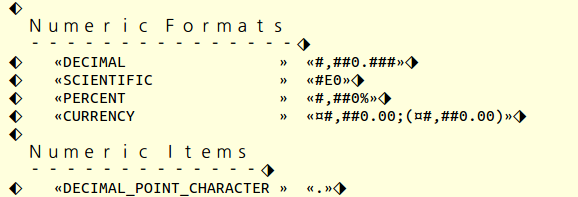
\includegraphics[angle=90,width=4in]{images/pseudo-dump.png}
\end{latexonly}
\begin{htmlonly}
    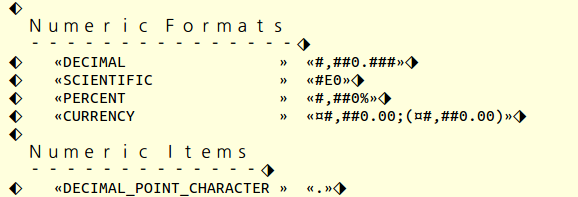
\includegraphics[width=4in]{images/pseudo-dump.png}
\end{htmlonly}
\end{center}
\caption{Display of the dump locale example with psuedo translation enabled.}
\label{fig:pseudo-dump}
\end{figure}

The example applications support pseudo translation via the \verb|-x|
options.

The GPS example patches enable pseudo translation for GPS via the command
line options \verb|--pseudo=|\textit{val}, where \textit{val} is one of
\texttt{u} (upper), \texttt{l} (lower), \texttt{h} (halfwidth) and
\texttt{e} (enclosed).  When halfwidth or enclosed mappings are used, the
``linkage'' between the standard menu item names and the localized names is
lost and additional menu items are created.  See figures~\ref{fig:gps-normal}
to~\ref{fig:gps-enclosed}.
\begin{figure}
\begin{center}
\begin{latexonly}
    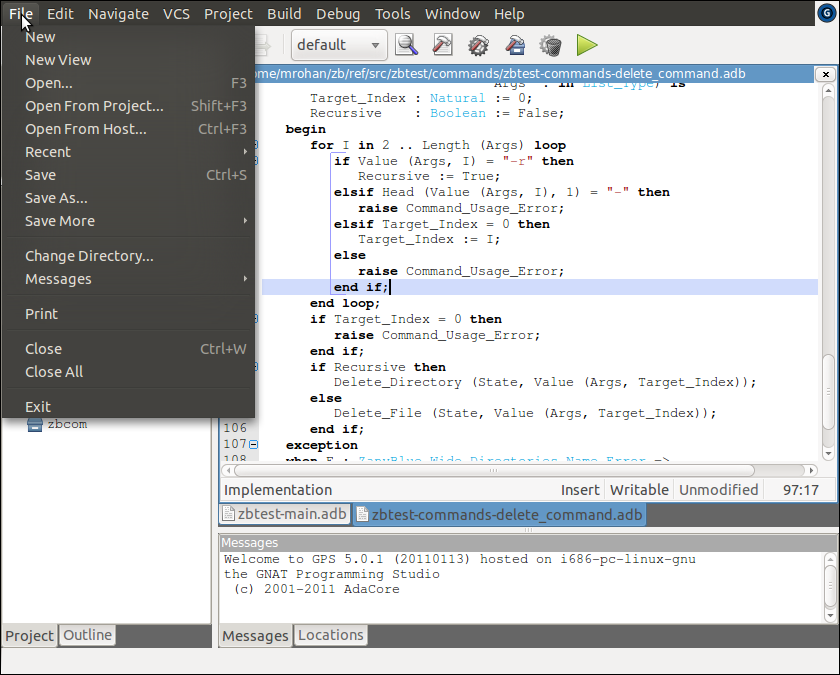
\includegraphics[angle=90,width=4in]{images/gps-normal.png}
\end{latexonly}
\begin{htmlonly}
    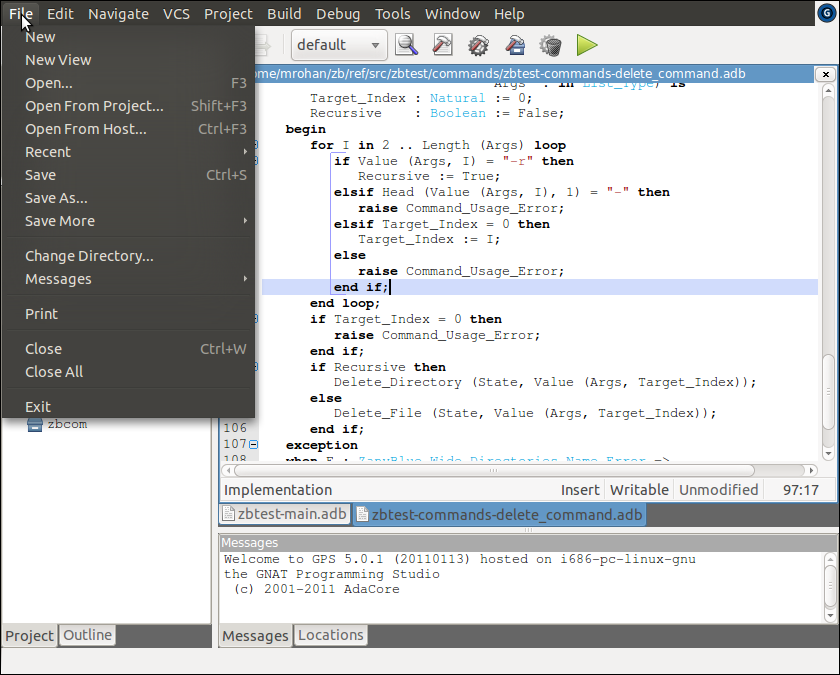
\includegraphics[width=4in]{images/gps-normal.png}
\end{htmlonly}
\end{center}
\caption{GPS display with no pseudo translation.}
\label{fig:gps-normal}
\end{figure}

\begin{figure}
\begin{center}
\begin{latexonly}
    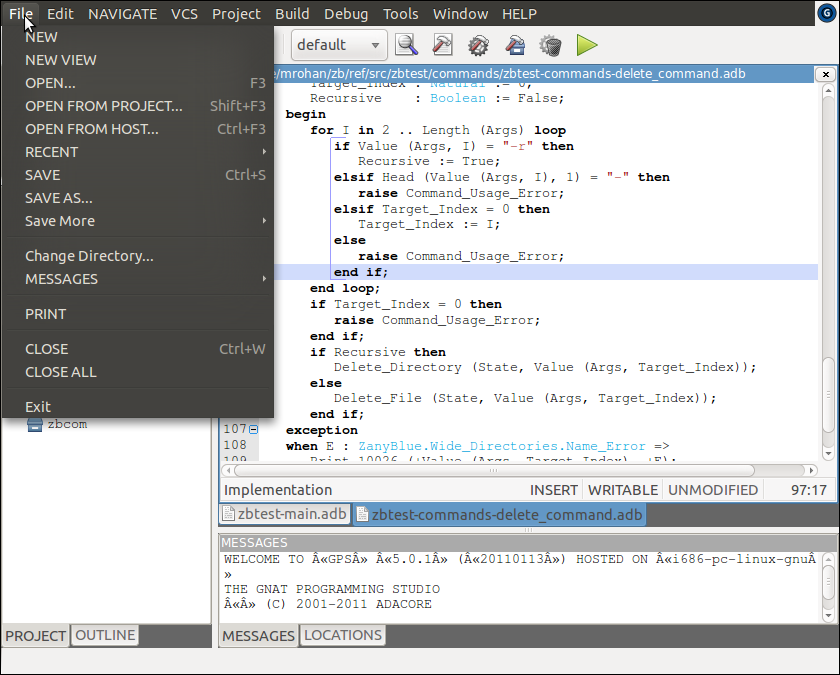
\includegraphics[angle=90,width=4in]{images/gps-upper.png}
\end{latexonly}
\begin{htmlonly}
    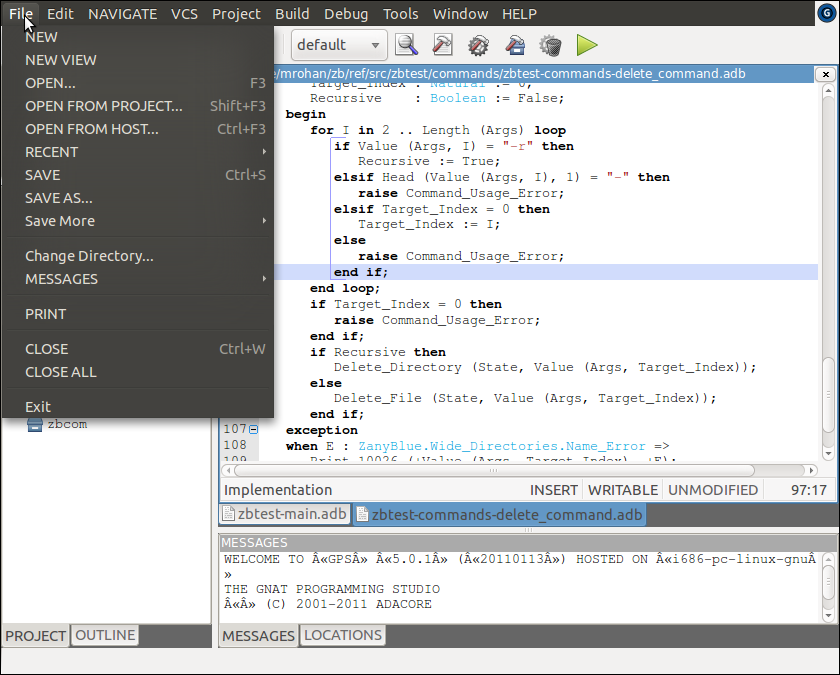
\includegraphics[width=4in]{images/gps-upper.png}
\end{htmlonly}
\end{center}
\caption{GPS display with uppercase pseudo translation.}
\label{fig:gps-upper}
\end{figure}

\begin{figure}
\begin{center}
\begin{latexonly}
    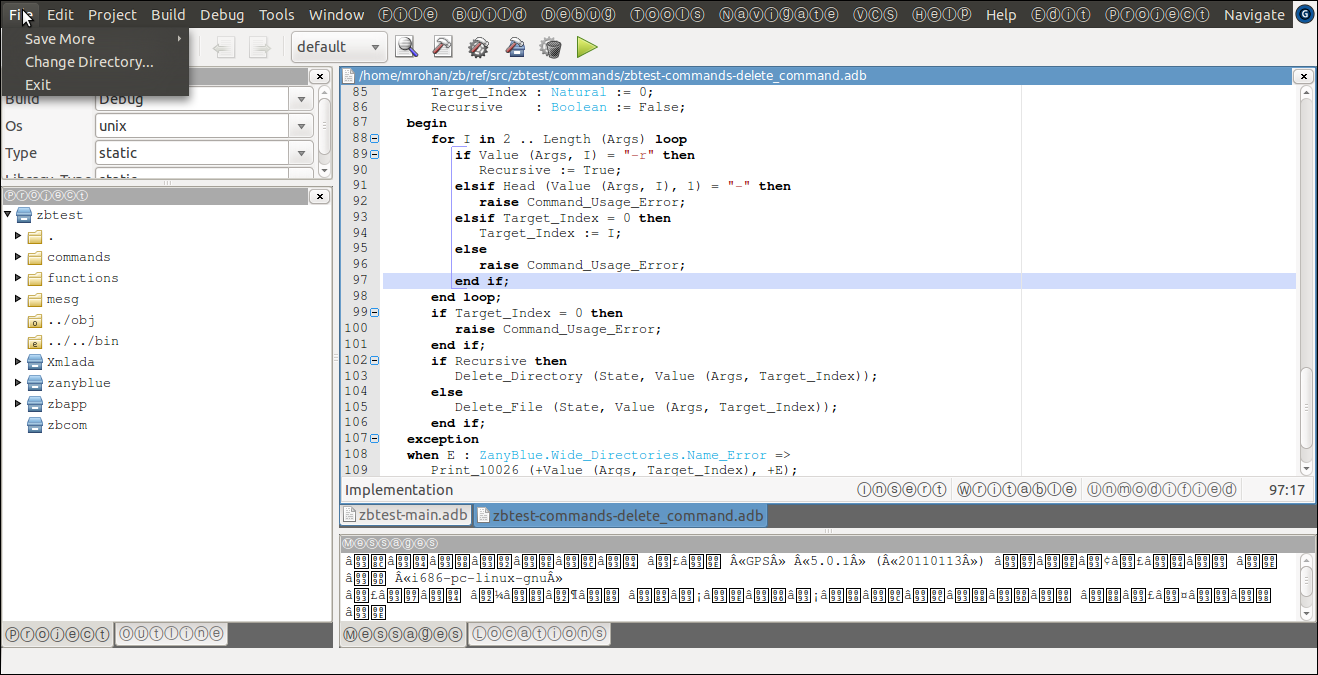
\includegraphics[angle=90,width=4in]{images/gps-enclosed.png}
\end{latexonly}
\begin{htmlonly}
    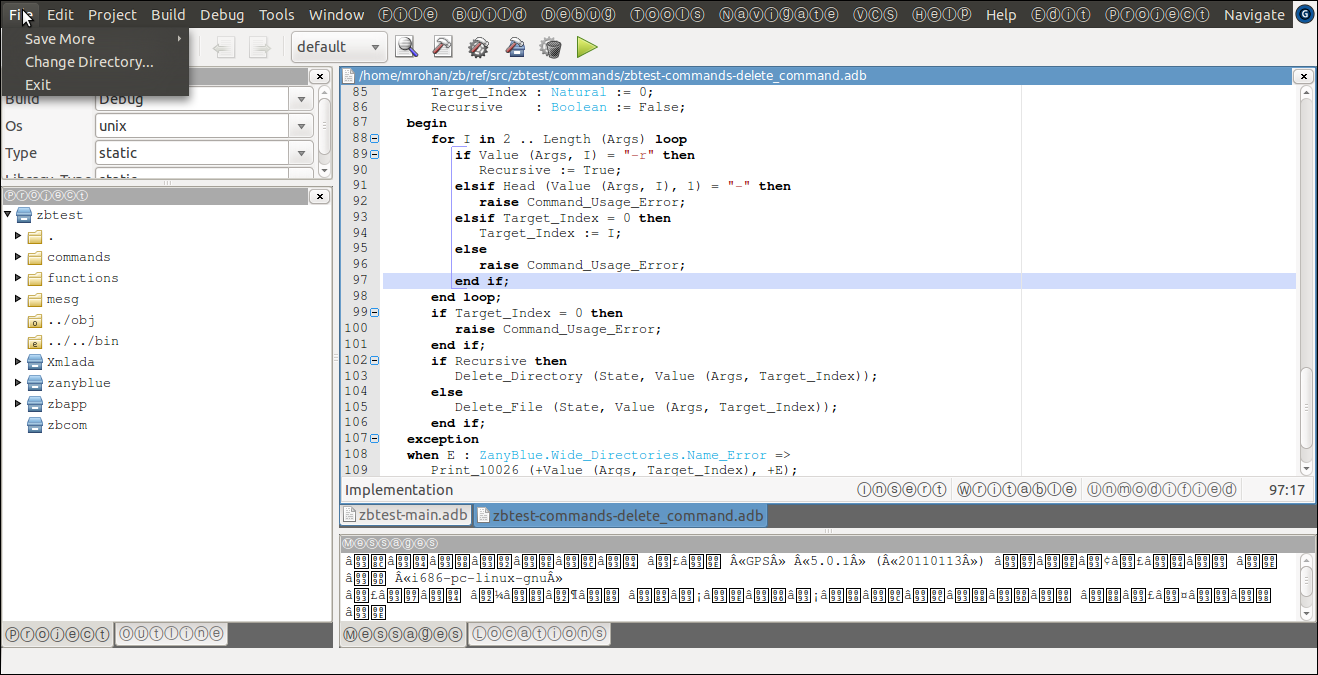
\includegraphics[width=4in]{images/gps-enclosed.png}
\end{htmlonly}
\end{center}
\caption{GPS display with enclosed pseudo translation.}
\label{fig:gps-enclosed}
\end{figure}

\section{Message `Metrics'}

Testing of internationalized applications (globalization, g11n, testing) is
slightly different from normal functional testing.  It is generally assumed
the core functionality of the application is not dependent on the the messaging.
Core testing is frequently driven by coverage data derived from the test
cases.  Performing testing in a globalized application to meet the same
coverage to generally not something that is needed.  The globalization
testing needs to verify the application is fully localized in the target
language and can handle localized input.  This is generally a subset of
the overall testing applied to an application.

To facilitate globalization testing, the library keeps track of the number
of times a message is used giving a coverage number, from a message point
of view.  The accumulated usage information can be saved to an XML file
using the \verb|Write_Usage| routines in the text \verb|Metrics| package.

%--------------------------------------------------------------------------
\section{The zbmcompile Utility}
\label{sec:zbmcompile}

The \verb|zbmcompile| utility compiles \texttt{.properties} files into
an Ada representation allowing easier access to the message text via
lookup in a catalog.

The simplest usage of the utility defines the name of the package to be
created and the facility to be compiled, e.g., for the moons example
application
\begin{xmpl}
\begin{verbatim}
   $ zbmcompile -i -v Moons_Messages moons
   This is ZBMCompile, Version 0.1.0 ALPHA (r1627) at 5:52 PM on 11/19/10
   Copyright (c) 2009-2010, Michael Rohan.  All rights reserved
   Loaded 16 messages for the facility "moons" (4 locales)
   Loaded 1 facilities, 4 keys, 4 locales and 16 messages
   Wrote the spec "Moons_Messages" to the file "moons_messages.ads"
   Wrote the body "Moons_Messages" to the file "moons_messages.adb"
   ZBMCompile completed at 5:52 PM on 11/19/10, elapsed time 0:00:00.263
\end{verbatim}
\end{xmpl}
Here the generated package \verb|Moons_Messages| is compiled from the
\texttt{.properties} files for the \verb|moons| facility in the current
directory.

\subsection{Controlling Status Output}

The \verb|zbmcompile| utility supports options to control the amount
of status information printed:
\begin{itemize}
\item[\texttt{-q}] Reduced the amount of output to just error and warning
                   messages.
\item[\texttt{-v}] Increase the amount of output generated.
\item[\texttt{-D}] Increase the amount of output to aid debugging.
\end{itemize}

\subsection{Definition of Properties Directory}

The default usage assumes the \texttt{.properties} files are located
in the current directory.   To locate the files in another directory,
the \verb|-d| option can be used, e.g.,
\begin{xmpl}
\begin{verbatim}
   $ zbmcompile -i -v -d mesg Moons_Messages moons
\end{verbatim}
\end{xmpl}
would locate the properties associated with the \verb|moons| facility
in the \verb|mesg| directory.

\subsection{Properties File Extension}

The default file extension used when locating properties files is
\texttt{.properties}.  This can be change using the \verb|-e| option.
E.g., to load all \texttt{.msg} files,
\begin{xmpl}
\begin{verbatim}
   $ zbmcompile -i -v -e .msg Moons_Messages moons
\end{verbatim}
\end{xmpl}

\subsection{Auto-Initialization}

The generate Ada code include an initialization routine which loads
the messages into a catalog (defaulting to the standard global
catalog).  The \verb|-i| option includes a call to this initialization
procedure in the body of the generated package.  This allows the
inclusion of the message in an application by simply including the
specification in a compilation unit, normally the main unit.  The
option also causes the inclusion of a warning suppression pragma
in the specification to allow compilation in a strict compilation
environment.

\subsection{Optimization of Messages}

When the \verb|zbmcompile| loads facilities in sequence which, in
general, distributes the messages associated with various locales.
The \verb|zbmcompile| optimize mode, the \verb|-O| option, performs
a second pass on the loaded messages gathering messages for each
locale together.  Since applications generally don't change locale
very often, if at all, having all the message strings for a locale
located in the same set of pages can improve performance.

For symmetry reasons, the \verb|-g| option is included which
disables optimization.

\subsection{Locale Selection}

Occasionally, only a subset of the \texttt{.properties} files should
be compiled into the generated Ada package.  This selection is supported
using the \verb|-B|, for base locale, and \verb|-L| options.  E.g., to
generate the Moons message package for just the base language, French and
German, the command would be
\begin{xmpl}
\begin{verbatim}
   $ zbmcompile -v -B -L fr -L de Moons_Messages moons
\end{verbatim}
\end{xmpl}
These option could be used to generate language packs, possibly via shared
library or dll implementations.

\subsection{Forced Compilation}

When testing using messages from Java projects, the message files will
frequently be found to contain errors from a \verb|zbmcompile| point of
view.  To force the generation of Ada in the context of input errors, the
\verb|-F| can be used.  Note, when used, there is no guarantee the resultant
generated Ada code will compile.

\subsection{Definition of External Initialization Routine}

The possible direction for Ada localization is to allow the loading of
language pack at run-time via shared library or dlls.  This has not been
investigated but in the context of dynamic loading of shared libraries or
dll's, having an initialization name that is well defined makes the
implementation easier.  To support this, the untested functionality of
supplying a linker name for the initialization routine is allowed via the
\verb|-x| option, e.g.,
\begin{xmpl}
\begin{verbatim}
   $ zbmcompile -v -B -x "moons_messages" Moons_Messages moons
\end{verbatim}
\end{xmpl}

\subsection{Generation of Accessor Packages}

The generation of message accessor packages creating routines for each
message defined with parameter lists matching the arguments defined by the
message text is controlled via the two options \verb|-a| and \verb|-G|.

The first style, \verb|-a|, generates all accessor style packages:
\begin{enumerate}
\item \verb|exceptions|, generate routines to raise exceptions with localized
     message strings (wide strings converted to UTF-8).
\item \verb|strings|, generate functions returning UTF-8 strings for the
     localized messages.
\item \verb|wstrings|, generate functions returning wide strings for the
     localized messages.
\item \verb|prints|, generate routines printing the localized messages to
     files as UTF-8 strings.
\item \verb|wprints|, generate routines printing the localized messages to
     files as wide strings (wide files).
\end{enumerate}

The \verb|-G| option allows the selection of individual accessor style
packages, e.g., for an application that only uses messages to raise
exceptions and print to wide files, the command line options would be
\verb|-G exceptions| and \verb|-G wprints|, i.e., the \verb|-G| option
can used multiple time on the same command line.

The packages generated are child packages of the primary package given on
the command line with names based on the facility name, e.g., if the
facility name is ``Moons'', the generated child packages would be
\begin{center}
\begin{tabular}{ll}
Style & Child Package Name\\\hline
\verb|exceptions| & \verb|Moons_Exceptions|\\
\verb|strings|    & \verb|Moons_Strings|\\
\verb|wstrings|   & \verb|Moons_Wide_Strings|\\
\verb|prints|     & \verb|Moons_Prints|\\
\verb|wprints|    & \verb|Moons_Wide_Prints|
\end{tabular}
\end{center}

\subsection{Output Directory}

By default, the generated packages are written to the current directory.  To
select a different directory, the \verb|-o| option can be used, e.g.,
\begin{xmpl}
\begin{verbatim}
   $ zbmcompile -o mesg Moons_Messages moons
\end{verbatim}
\end{xmpl}
would write the packages to the \verb|mesg| directory.  The directory must
already exist.

\subsection{Adjusting the Generated Code}

The \verb|zbmcompile| command has a number of options used to adjust the
generated code.

\subsubsection{Comments for Accessors}

By default, the generated routines for accessors include the base message
text as a comment.  This allows the display of the text of the messages within
GPS and makes browsing the source easier.  These comments can be suppressed
using the \verb|-C| option.  One reason to suppress these comments would be
to minimize recompilations when updating messages.  The \verb|zbmcompile|
command will only create new source files if the generated contents differs
from the existing files (or the files currently doesn't exist).  With
comments suppressed, updating message strings would only result in the update
to the primary package body requiring, in general, a single recompilation and
re-link of an application.  With comment enabled, the accessor spec files
would be updated resulting in larger recompilations.

\subsubsection{Argument Modes}

The default code generated does not include the \verb|in| keyword for in
routine arguments.  Some code bases might have style rules requiring explicit
use of this keyword.  To require the generated code include this keyword, the
\verb|-m| option can be used.

\subsubsection{Positional Elements}

The generated code includes a number of initialized tables (arrays).  The
default style for such tables is simply to list the entries using implicit
index association.  Again, some code bases might require that explicit
numbering of such code.  This can be enabled using the \verb|-p| command
line option.  E.g., instead of
\begin{xmpl}
\begin{verbatim}
   Facilities : constant ZT.Constant_String_List (1 .. 7) := (
                   Facility_1'Access,
                   Facility_2'Access,
   ...
\end{verbatim}
\end{xmpl}
the generated code would be
\begin{xmpl}
\begin{verbatim}
   Facilities : constant ZT.Constant_String_List (1 .. 7) := (
                   1 => Facility_1'Access,
                   2 => Facility_2'Access,
   ...
\end{verbatim}
\end{xmpl}

\subsubsection{Output Line Lengths}

The generated code keeps within the standard 80 column style for source files.
There are two control parameters which can be used as arguments to the \verb|-T|
command line option to adjust this for selected items:
\begin{enumerate}
\item The accumulated message strings are stored as a single constant string
      initialized using a multi-line string.  The length of the substrings
      written per line can be controlled using the command line \verb|pool|
      item with an integer value, e.g., \verb|-T pool 30| to reduce the size.
\item The base message text written as a comment on accessors is wrapped to
      ensure the 80 column limit is not exceeded.   This results in wrapping
      within words.  To increase the limit for messages, use the \verb|comment|
      item, e.g., \verb|-T comment 120|.  Accessor comments include breaks
      for messages with new lines.
\end{enumerate}

\subsection{Consistency Checks}

Localized messages are cross checked with the base locale messages to ensure
they are consistent, i.e., it is an error for a localized message to refer
to an argument not present in the base message.

There are two options that control the consistency checks performed
\begin{enumerate}
\item \verb|-u|, disable the consistency checks.  This is a rather dangerous
      thing to do and should be avoided.
\item \verb|-r| define the base locale.  Normally the base locale messages
      are in the properties file without a locale, i.e., the root locale.
      Some applications might choose to use explicit locale naming for all
      properties files.  The \verb|-r| option can be used to designate which
      of the available locales is the base locale.
\end{enumerate}

\subsection{Selection of Source Locale}

The source locale for the base properties file can be specified using the
\verb|-s| option.  See \ref{sec:sourcelocale} for details on this functionality.

\subsection{Stamp File}

For Makefile base builds, dependency checking is simplified if a single fixed
named file can be used rather than the set of generated spec and body files
normally created by \verb|zbmcompile|.  The \verb|-S| option allows the
definition of a simple time stamp file which is updated whenever the
\verb|zbmcompile| command is run.  This file can be used to define built
dependencies in Makefiles.
